\documentclass[11pt,a4paper]{beamer}
\mode<presentation>
\usepackage[spanish]{babel}
\usepackage[utf8]{inputenc}
\usepackage{amsmath}
\usepackage{amsfonts}
\usepackage{amssymb}
\usepackage{graphicx}
\usepackage{cprotect}
\usepackage{siunitx}
\usepackage{listings}
\usepackage{tikz}
\usetikzlibrary{arrows,babel,backgrounds,fit,patterns,petri,positioning,shapes}

\tikzstyle{core}=[
	rectangle,
	rounded corners,
	draw=black,
	minimum size=40]

\tikzstyle{perif}=[
	core,
	minimum height=20]

\tikzstyle{contenedor}=[
	rectangle,
	draw=black]

\tikzstyle{exterior}=[
	rectangle,
	draw=black,
	minimum size=40]

\tikzstyle{bloque}=[
	exterior,
	align=center,
	minimum size=60,
	text width=60]

\tikzstyle{pid}=[
	draw=black,
	align=center,
	rectangle,
	rounded corners,
	minimum width=20,
	minimum height=110,
	pattern=north east lines,
	pattern color=black!35]

\tikzstyle{dir}=[
	draw,
	rectangle,
	rounded corners,
	minimum width=20,
	minimum height=110,
	align=center]

\tikzstyle{data}=[
	draw=black,
	align=center,
	rectangle,
	rounded corners,
	minimum width=120,
	minimum height=110,
	fill=black!05]

\tikzstyle{crc}=[
	draw=black,
	align=center,
	rectangle,
	rounded corners,
	minimum width=20,
	minimum height=110,
	pattern=dots,
	pattern color=black!25]

\tikzstyle{buf}=[
	core,
	text width=55,
	align=center,
	fill=white]
	
\tikzstyle{obuf}=[
	buf,
	node distance=.7,
	fill=white]
	
\tikzstyle{env}=[
	fill=black!20]

\tikzstyle{moore}=[
	rectangle,
	draw=black,
	minimum height=30,
	text width=80,
	align=left]
	
\tikzstyle{mealy}=[
	rectangle,
	rounded corners=6,
	draw=black,
	text width=80,
	align=left,
	minimum height=40]

\tikzstyle{ask}=[
	diamond,
	text width=50,
	draw=black,
	align=center]
	
\tikzstyle{simple}=[
	rectangle,
	draw=black,
	minimum height=220,
	text width=65,
	align=center]

\newcommand{\epg}[3]{
	Buffer {#1}\\
	[44pt]EP{#2}\\
	[44pt]{#3} Bytes}

\newcommand{\ep}[3]{
	Buffer {#1}\\
	[8pt]EP{#2}\\
	[8pt]{#3} Bytes}

\usetheme[secheader]{Boadilla}
% diagramas temporales
\newcounter{wavecount}

\newcommand{\newwave}[1]{
	\path (0,\value{wavecount}) node[text width=45,anchor=east,align=right]{#1} node[coordinate](t_cur){};
	\draw (0,\value{wavecount}+.3) --++(.2,0);
	\draw (0,\value{wavecount}-.3) --++(.2,0);
	\path (t_cur) --++(.3,0)node[coordinate](t_cur){};
	\addtocounter{wavecount}{-1}}

\newcommand*{\bit}[2]{
	\draw (t_cur) -- ++(0.1,.6*#1-.3) -- ++(#2-.2,0) -- ++(+.1,.3-.6*#1)
	node[coordinate] (t_cur) {};}
%diagramas temporales


\graphicspath{{./img/}}

\author[E. Barragán]{Edwin Barragán\\ \texttt{edwin.barragan@cab.cnea.gov.ar}}
\title{Temas Específicos de Electrónica Digital I}
\subtitle{Comunicación USB 2.0 para aplicaciones cientificas basadas en FPGA}
\institute[UNSJ-FI]{Universidad Nacional de San Juan\\Facultad de Ingeniería}

\AtBeginSubsection[]
{
	\begin{frame}<beamer>{Agenda}
		\tableofcontents[sections=\thesection,currentsubsection]
	\end{frame}
}

\begin{document}
%TODO tengo 18 filminas que no deben ser consideradas
	\titlepage
	\begin{frame}[c]{Una comunicación USB\\para aplicaciones científicas basadas en FPGA}
		\framesubtitle{Preámbulo}
		\centering
		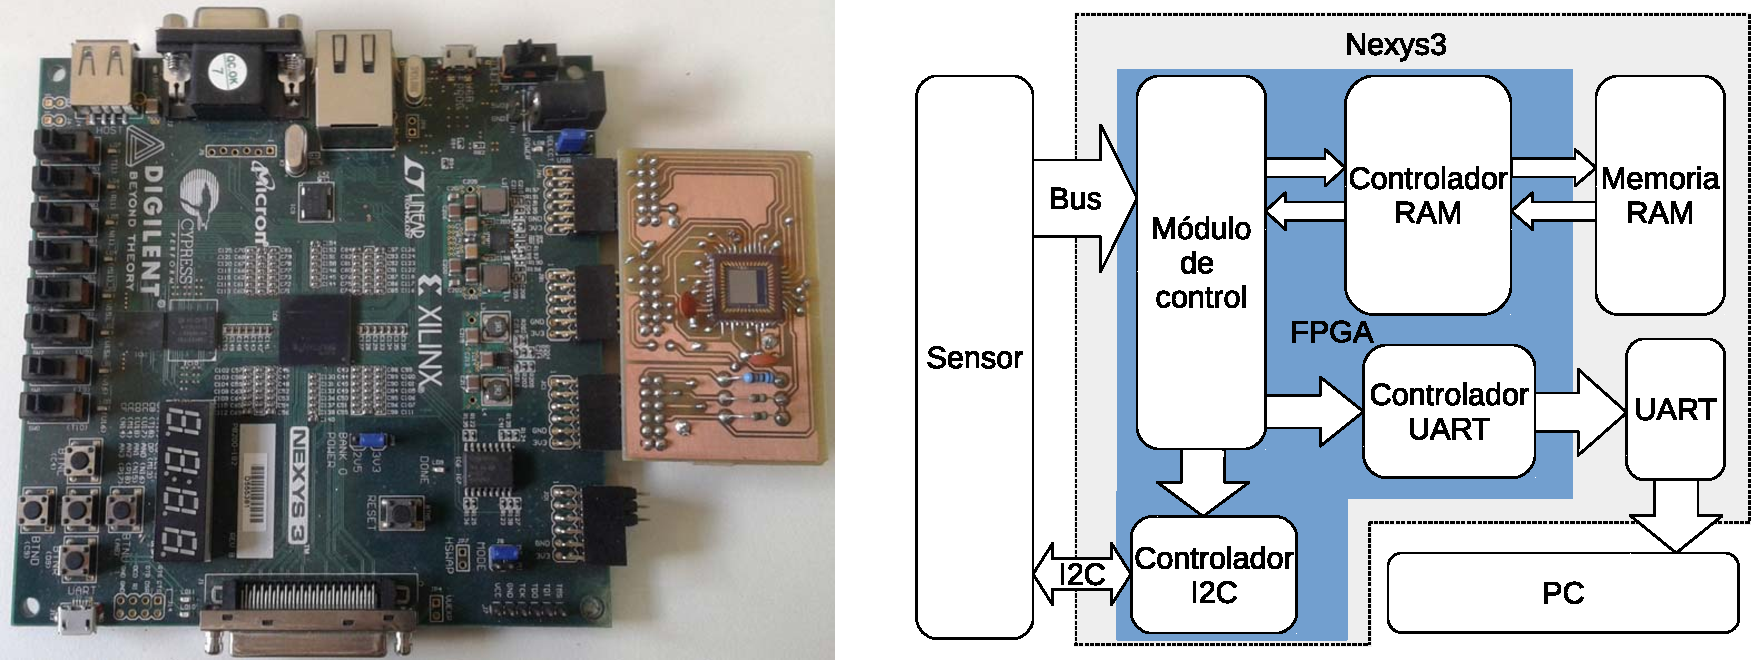
\includegraphics[width=0.9\paperwidth]{01motivacion}
	\end{frame}
	\begin{frame}{Agenda}
		\tableofcontents[hideallsubsections]
	\end{frame}
	\begin{frame}{Agenda}
		\tableofcontents[sections={1,2}]
	\end{frame}
	\begin{frame}{Agenda}
		\tableofcontents[sections={3,4}]
	\end{frame}
	\section{Introducción}
		\subsection{Motivación}
			\begin{frame}{La producción de información científica}
				\begin{itemize}
					\item Los avances en las escalas de integración de circuitos permiten desarrollar sensores que recolectan mayor volumen de datos.
					\item Los nuevos sensores necesitan nuevos circuitos adicionales que les permitan adquirir datos y controlar su funcionamiento.
					\item La utilización de FPGA es muy útil para sintetizar circuitos digitales.
					\item Los datos deben ser procesados para transformase en información.
					\item Los datos se deben transmitir desde los sistemas generadores a los sistemas procesadores.
				\end{itemize}
			\end{frame}
			%ACA me gustaría poner un frame donde se explique en forma gráfica lo de los sitemas procesadores y sistemas generadores
			\begin{frame}{La necesidad de una comunicación\\entre un FPGA y una PC}
				\begin{itemize}
					\item Las computadoras son herramientas muy útiles para procesar datos.
					\item Los FGPAs pueden operar a altas velocidades y utilizar puertos paralelos.
					\item Es de utilidad una comunicación entre las PCs y las aplicaciones que utilizan FPGA para la implementación de circuitos.
					\item USB es una opción robusta, con ancho de banda suficiente para transmitir imágenes e incorporada en cualquier PC moderna.
				\end{itemize}
			\end{frame}
		\subsection{Objetivos}
			\begin{frame}{Objetivos}
				\begin{itemize}
					\item Objetivo General
					\begin{itemize}
						\item Realizar una comunicación entre un FPGA y una PC mediante USB 2.0
					\end{itemize}
					\item Objetivos Particulares
					\begin{itemize}
						\item Comprender el funcionamiento del kit de desarrollo CY3684 y el framework provisto por Cypress.
						\item Configurar el chip CY7C68014A, incorporado en el kit de desarrollo anterior.
						\item Sintetizar un circuito en VHDL que sea capaz de interactuar con las memorias FIFO de la interfaz.
						\item Sintetizar circuitos de prueba para Test Bench.
						\item Validar el funcionamiento.
					\end{itemize}
				\end{itemize}
			\end{frame}
		\subsection{Bus Serial Universal}
			\begin{frame}{USB - Bus Serial Universal}
					El Bus Serial Universal o USB es un sistema de comunicación pensado, en su concepción original, para conectar periféricos a una PC.\\
					Los objetivos perseguidos por norma son:

				\begin{itemize}
					\item Conexión de teléfonos a la PC.
					\item Facilidad de uso.
					\item Proveer un puerto de expansión para periféricos.
					\item<2-> \alert {Mayor rendimiento}
					\item<2-> \alert {Mayor ancho de banda}
%					\item Topológicamente, posee una estructura mestro-esclavo, en forma de árbol, donde el nodo principal es el Host, el resto de los nodos está implementado con Hubs y cada dispositivo es un esclavo.
%					\item Mecánicamente, 
				\end{itemize}
				
				\only <2-> {La respuesta a esta demanda fue agregar una nueva velocidad de 480 Mbit/s.}
				
			\end{frame}
			\begin{frame}{USB - Topología}
				\centering
				\begin{itemize}
					\item \only<1> {Física} \only<2> {Lógica}
				\end{itemize}
				\only<1>{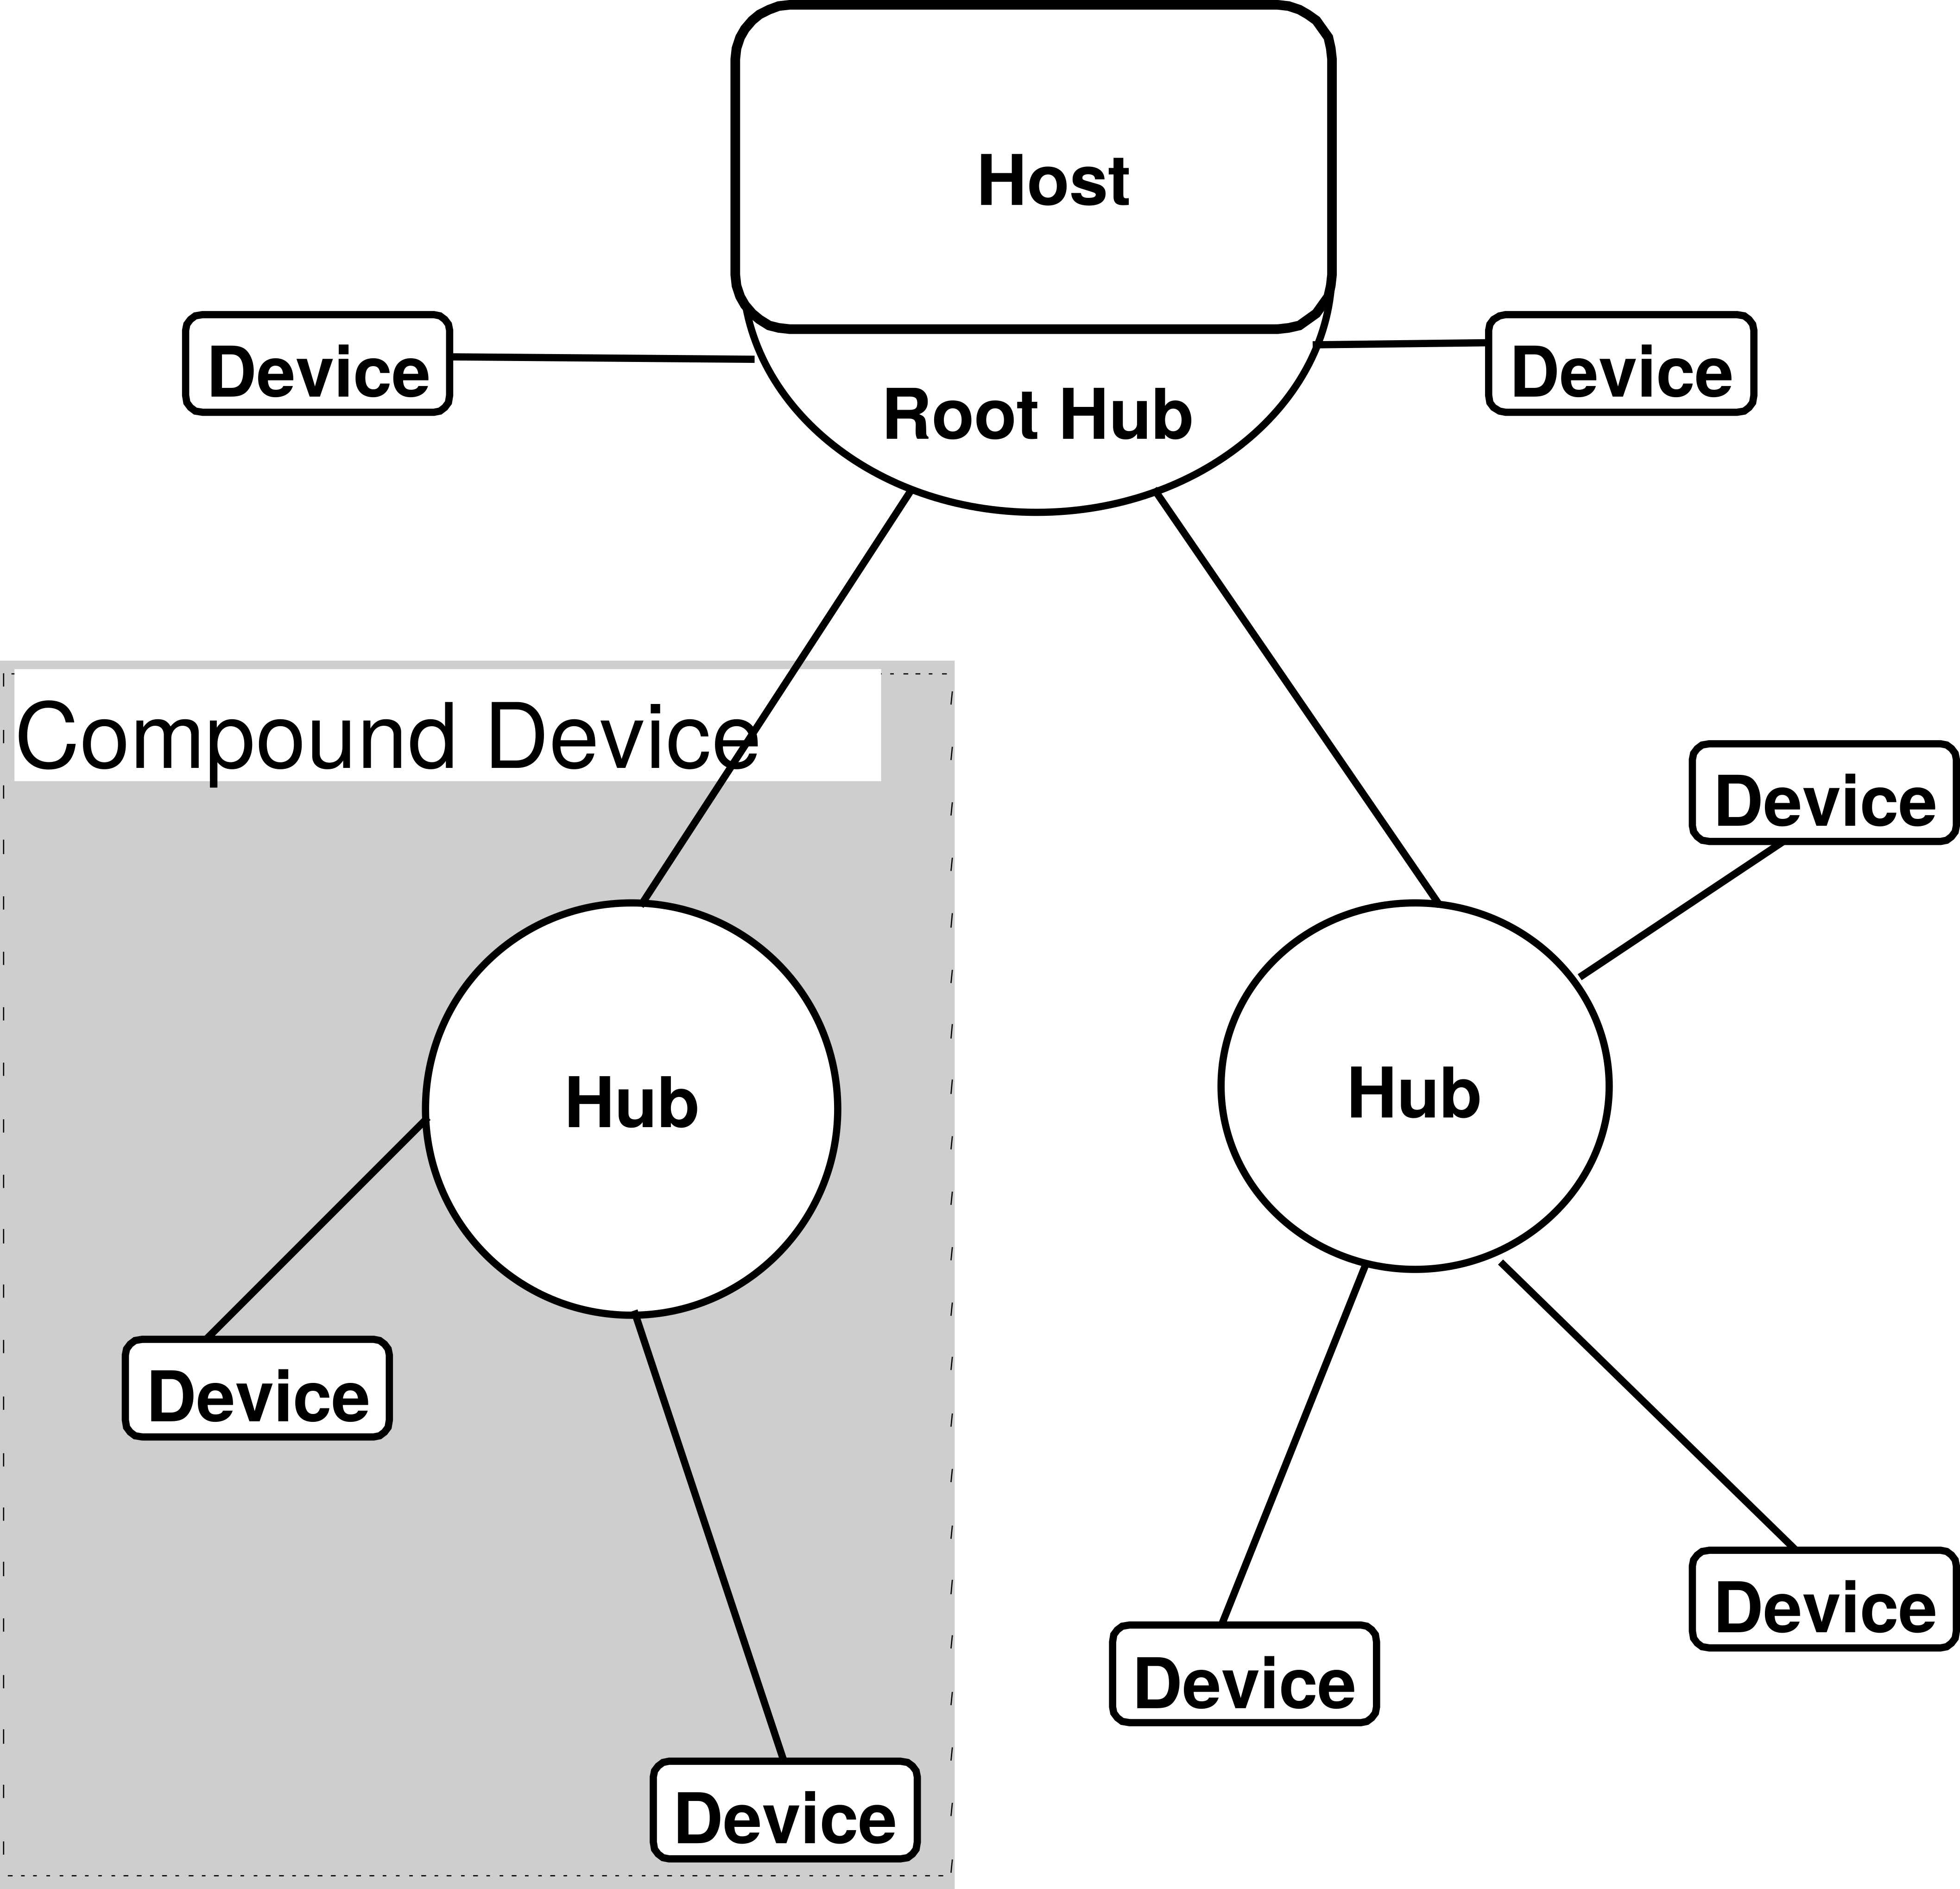
\includegraphics[width=0.6\textwidth]{topofisica.png}}
				\only<2>{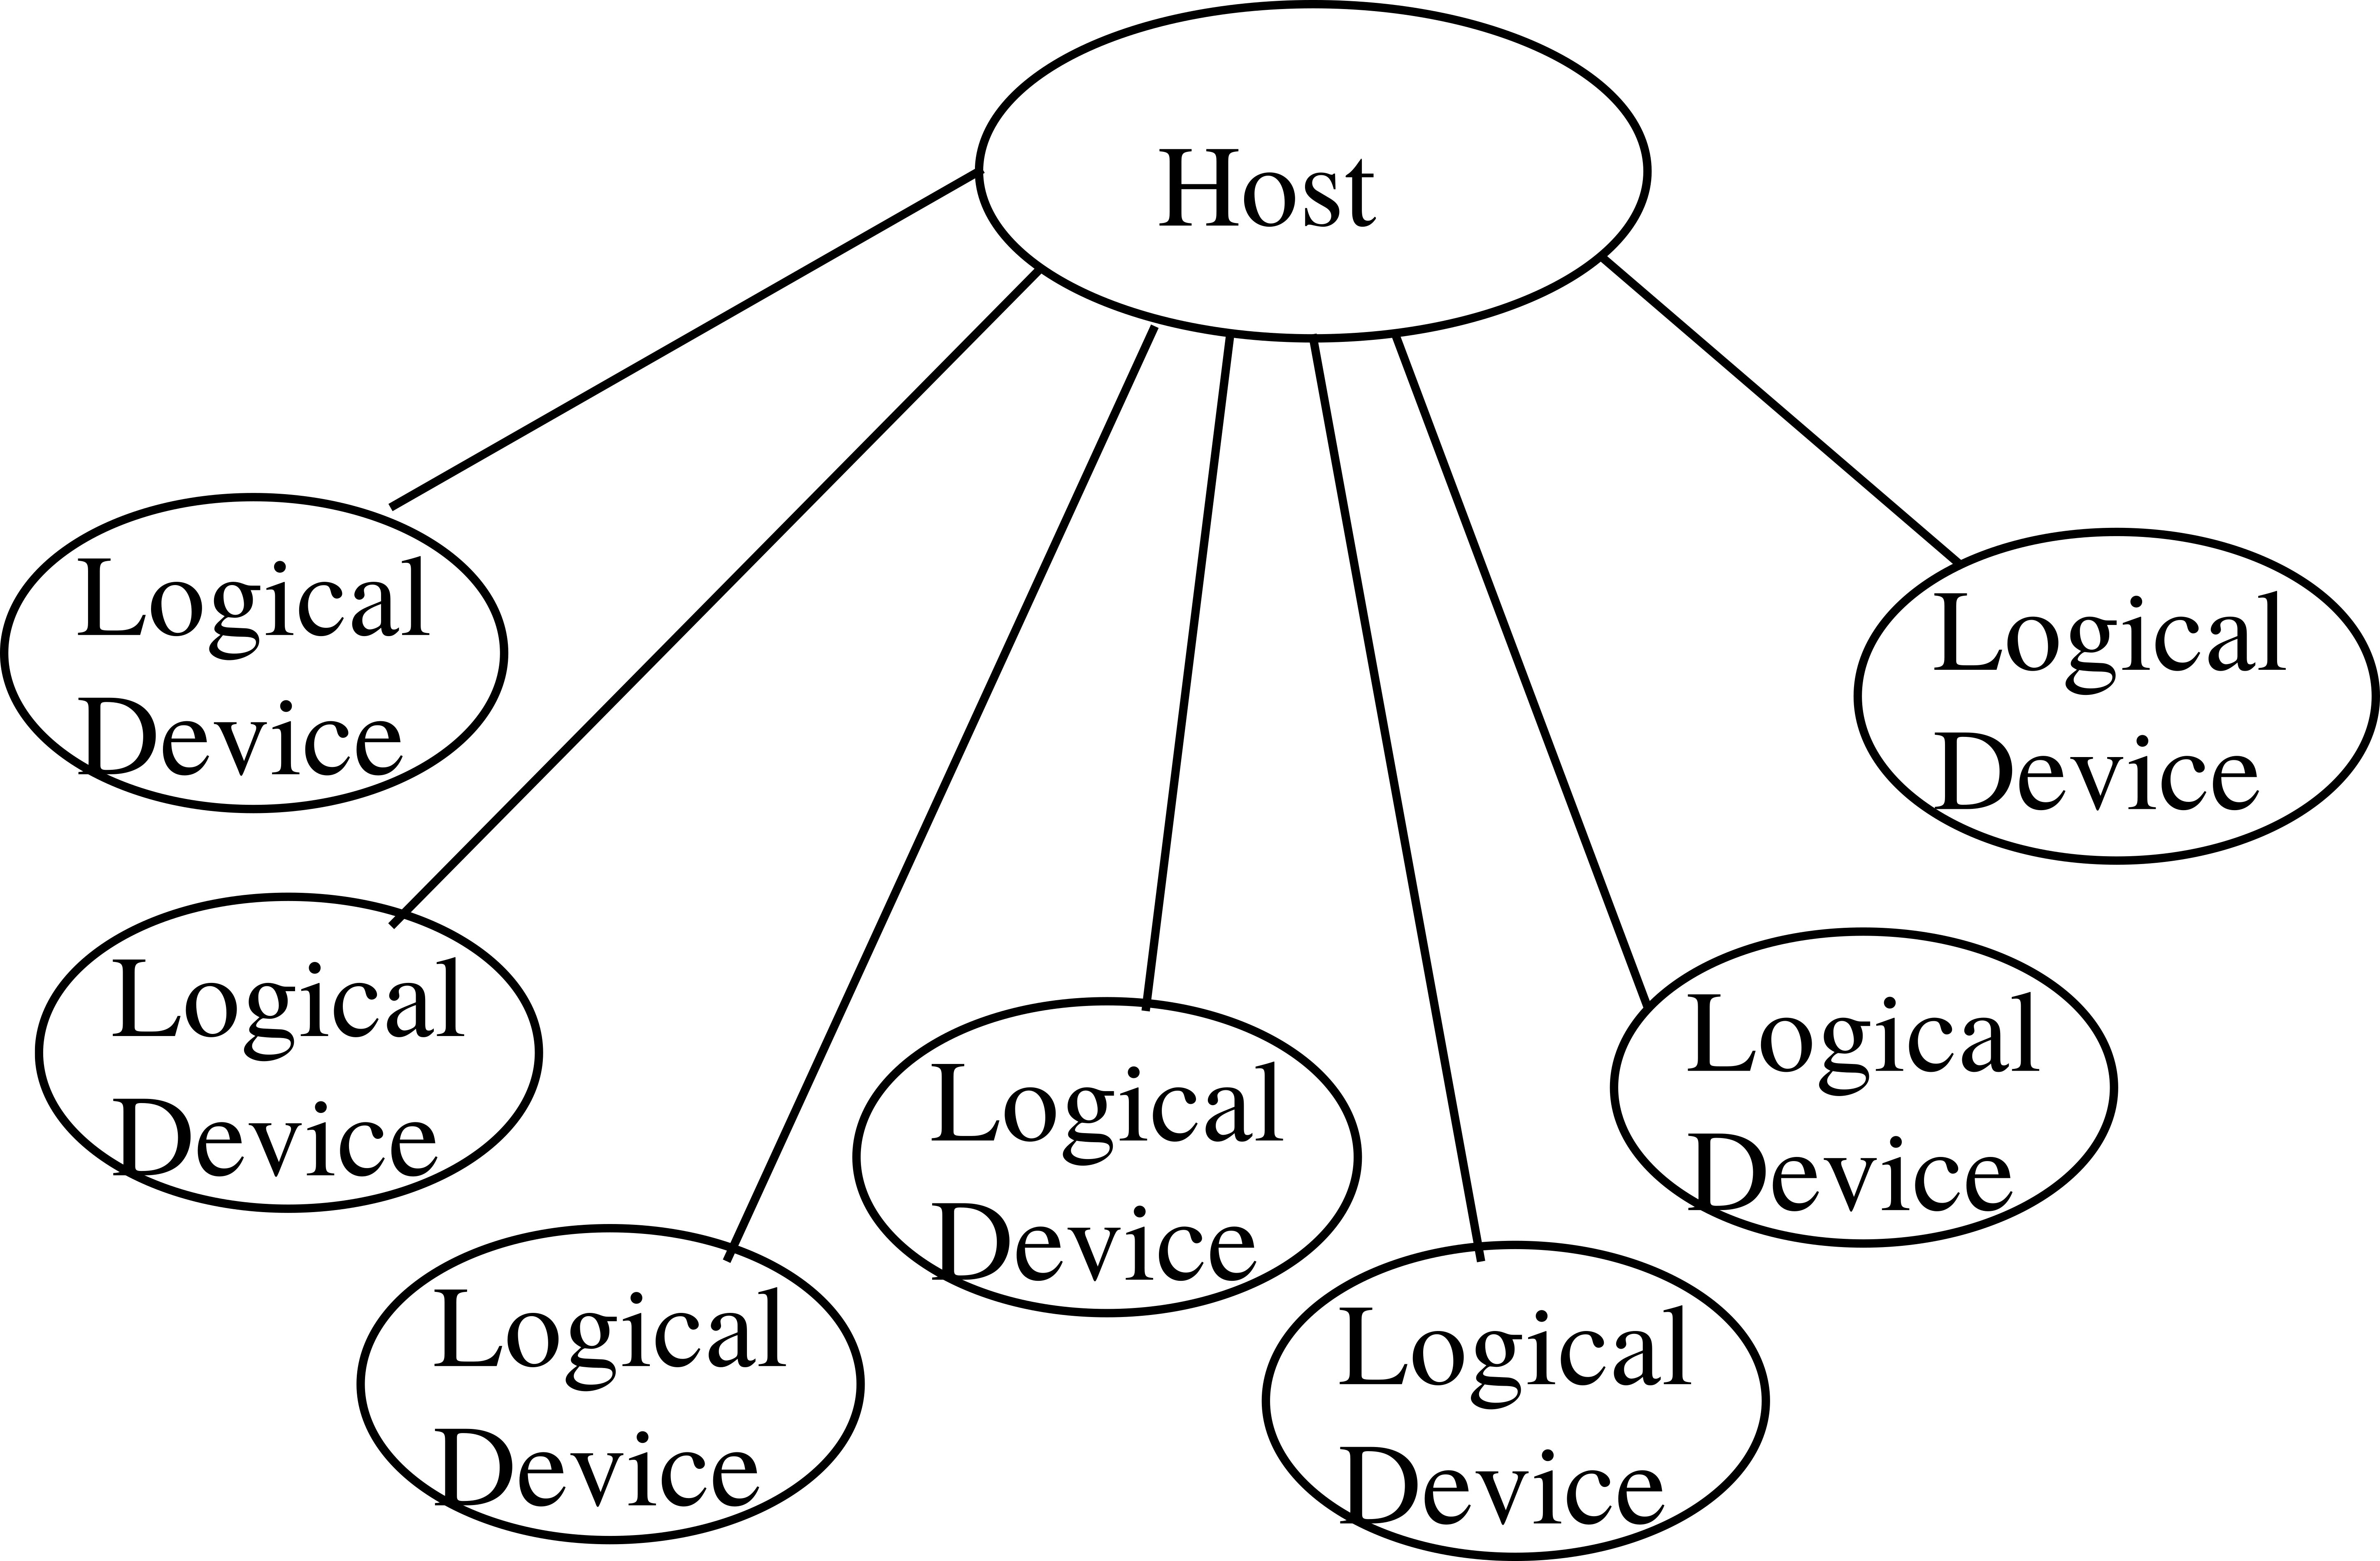
\includegraphics[width=0.8\textwidth]{topologica.png}}
			\end{frame}
			\begin{frame}{USB - Flujo de datos}
				\centering
				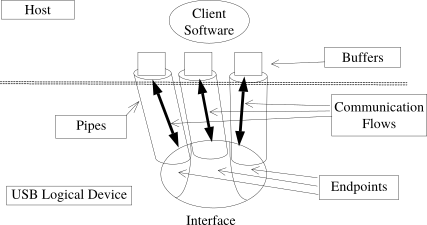
\includegraphics[width=0.8\textwidth]{complogicos.png}
			\end{frame}
			\begin{frame}{USB - Tipos de paquetes}
				\begin{itemize}
					\item Paquetes Token
					\item Paquetes de Datos
					\item Paquetes de Handshake
					\item Paquetes Especiales
				\end{itemize}
			\end{frame}
			\begin{frame}{USB - Trama de paquetes}
				\begin{itemize}
					\item Entrada de Paquetes al Host
						\begin{center}
							\begin{tikzpicture}[scale=.6\textwidth/\paperwidth,>=latex]
								\begin{scope}
									\begin{scope}[transform shape,node distance=.15]
										\node[pid]	(pidtok)	{\bf{I}\\\bf{N}\\\ \\T\\o\\k.};
										\node[dir]	(adtok)	[right=of pidtok]	{D\\i\\r.};
										\node[dir]	(eptok)	[right=of adtok]	{E\\x\\t\\r.};
										\node[crc]	(crc5)	[right=of eptok]	{C\\R\\C\\5};
									\end{scope}
									\begin{scope}
										\node[exterior,minimum size=0,inner sep=1,fit=(adtok)(eptok)](tokad){};
										\node[below=.01 of tokad.south,align=center,transform shape] (texttok){Paquete\\Token};
										\node[exterior,inner sep=1,fit=(pidtok)(tokad)(crc5)(texttok)](pkttok){};
									\end{scope}
									\begin{scope}[transform shape,node distance=.15]
										\node[pid,node distance=.4]	(piddat)	[right=of crc5]{D\\a\\t\\a\\\\P\\I\\D};
										\node[data]	(data)	[right=of piddat]	{Datos\\útiles};
										\node[crc]	(crc16)	[right=of data]	{C\\R\\C\\1\\6};
									\end{scope}
									\begin{scope}
										\node[below=.01 of data.south,align=center,transform shape] (textdat){Paquete\\de Datos};
										\node[exterior,inner sep=2,fit=(piddat)(data)(crc16)(textdat)]{};
									\end{scope}
										\begin{scope}[transform shape,node distance=.15]
										\node[pid,node distance=1.3]	(hspid)	[right=of crc16]%.north east,anchor=south east]
										{H\\S\\\ \\P\\I\\D};
									\end{scope}
									\begin{scope}
										\node[below=.01 of hspid.south,align=center,transform shape] (texths){Paquete\\de Handshake};
										\node[exterior,inner sep=2,fit=(hspid)(texths)]{};
									\end{scope}
								\end{scope}
							\end{tikzpicture}
						\end{center}
					\item Salida de Paquetes hacia periféricos
						\begin{center}
							\begin{tikzpicture}[scale=.6\textwidth/\paperwidth,>=latex]
								\begin{scope}
									\begin{scope}[transform shape,node distance=.15]
										\node[pid]	(pidtok)	{\bf{O}\\\bf{U}\\\bf{T}\\\ \\T\\o\\k.};
										\node[dir]	(adtok)	[right=of pidtok]	{D\\i\\r.};
										\node[dir]	(eptok)	[right=of adtok]	{E\\x\\t\\r.};
										\node[crc]	(crc5)	[right=of eptok]	{C\\R\\C\\5};
									\end{scope}
									\begin{scope}
										\node[exterior,minimum size=0,inner sep=1,fit=(adtok)(eptok)](tokad){};
										\node[below=.01 of tokad.south,align=center,transform shape] (texttok){Paquete\\Token};
										\node[exterior,inner sep=1,fit=(pidtok)(tokad)(crc5)(texttok)](pkttok){};
									\end{scope}
									\begin{scope}[transform shape,node distance=.15]
										\node[pid,node distance=.4]	(piddat)	[right=of crc5]{D\\a\\t\\a\\\\P\\I\\D};
										\node[data]	(data)	[right=of piddat]	{Datos\\útiles};
										\node[crc]	(crc16)	[right=of data]	{C\\R\\C\\1\\6};
									\end{scope}
									\begin{scope}
										\node[below=.01 of data.south,align=center,transform shape] (textdat){Paquete\\de Datos};
										\node[exterior,inner sep=2,fit=(piddat)(data)(crc16)(textdat)]{};
									\end{scope}
									\begin{scope}[transform shape,node distance=.15]
										\node[pid,node distance=1.3]	(hspid)	[right=of crc16]%.north east,anchor=south east]
									{H\\S\\\ \\P\\I\\D};
									\end{scope}
									\begin{scope}
										\node[below=.01 of hspid.south,align=center,transform shape] (texths){Paquete\\de Handshake};
										\node[exterior,inner sep=2,fit=(hspid)(texths)]{};
									\end{scope}
								\end{scope}
							\end{tikzpicture}
						\end{center}
				\end{itemize}
			\end{frame}
			\begin{frame}{USB - Conexión mecánica}
				\only<1>{
					\begin{itemize}
						\item La conexión mecánica posee dos pares de conductores: uno de alimentación ($V_{BUS}$ y GROUND) y otro de datos diferenciales(D+ y D-). Además posee diferentes tipos de fichas de conexión.
						\item Los conectores poseen diferencia en los extremos, a fin de identificar el extremo que va hacia el Host (tipo A) y el extremo que va hacia los dispositivos (tipo B, mini USB, micro USB)
					\end{itemize}}
				\only<2>{
					\begin{figure}
						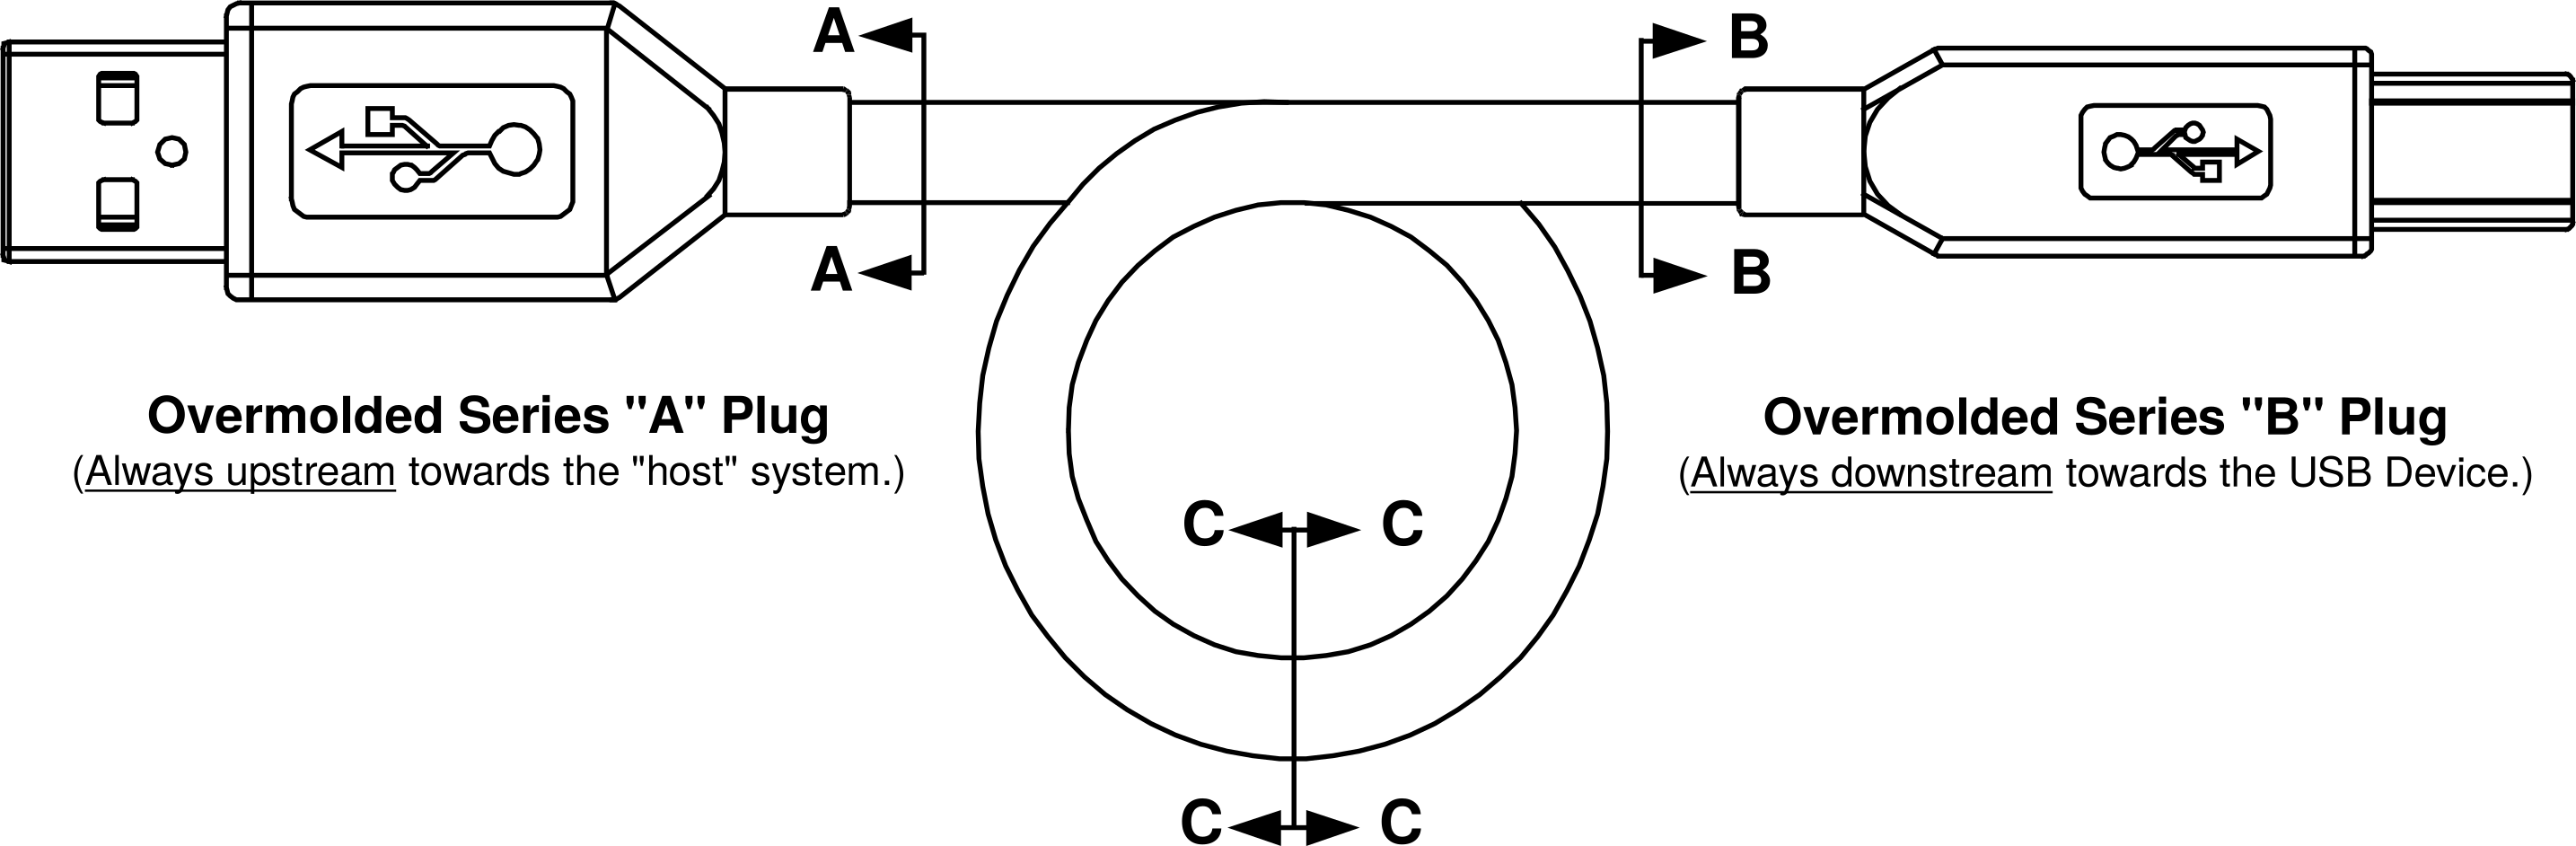
\includegraphics[width=.9\textwidth]{usbcableb.png}
					\end{figure}}
				\only<3>{
					\begin{figure}
						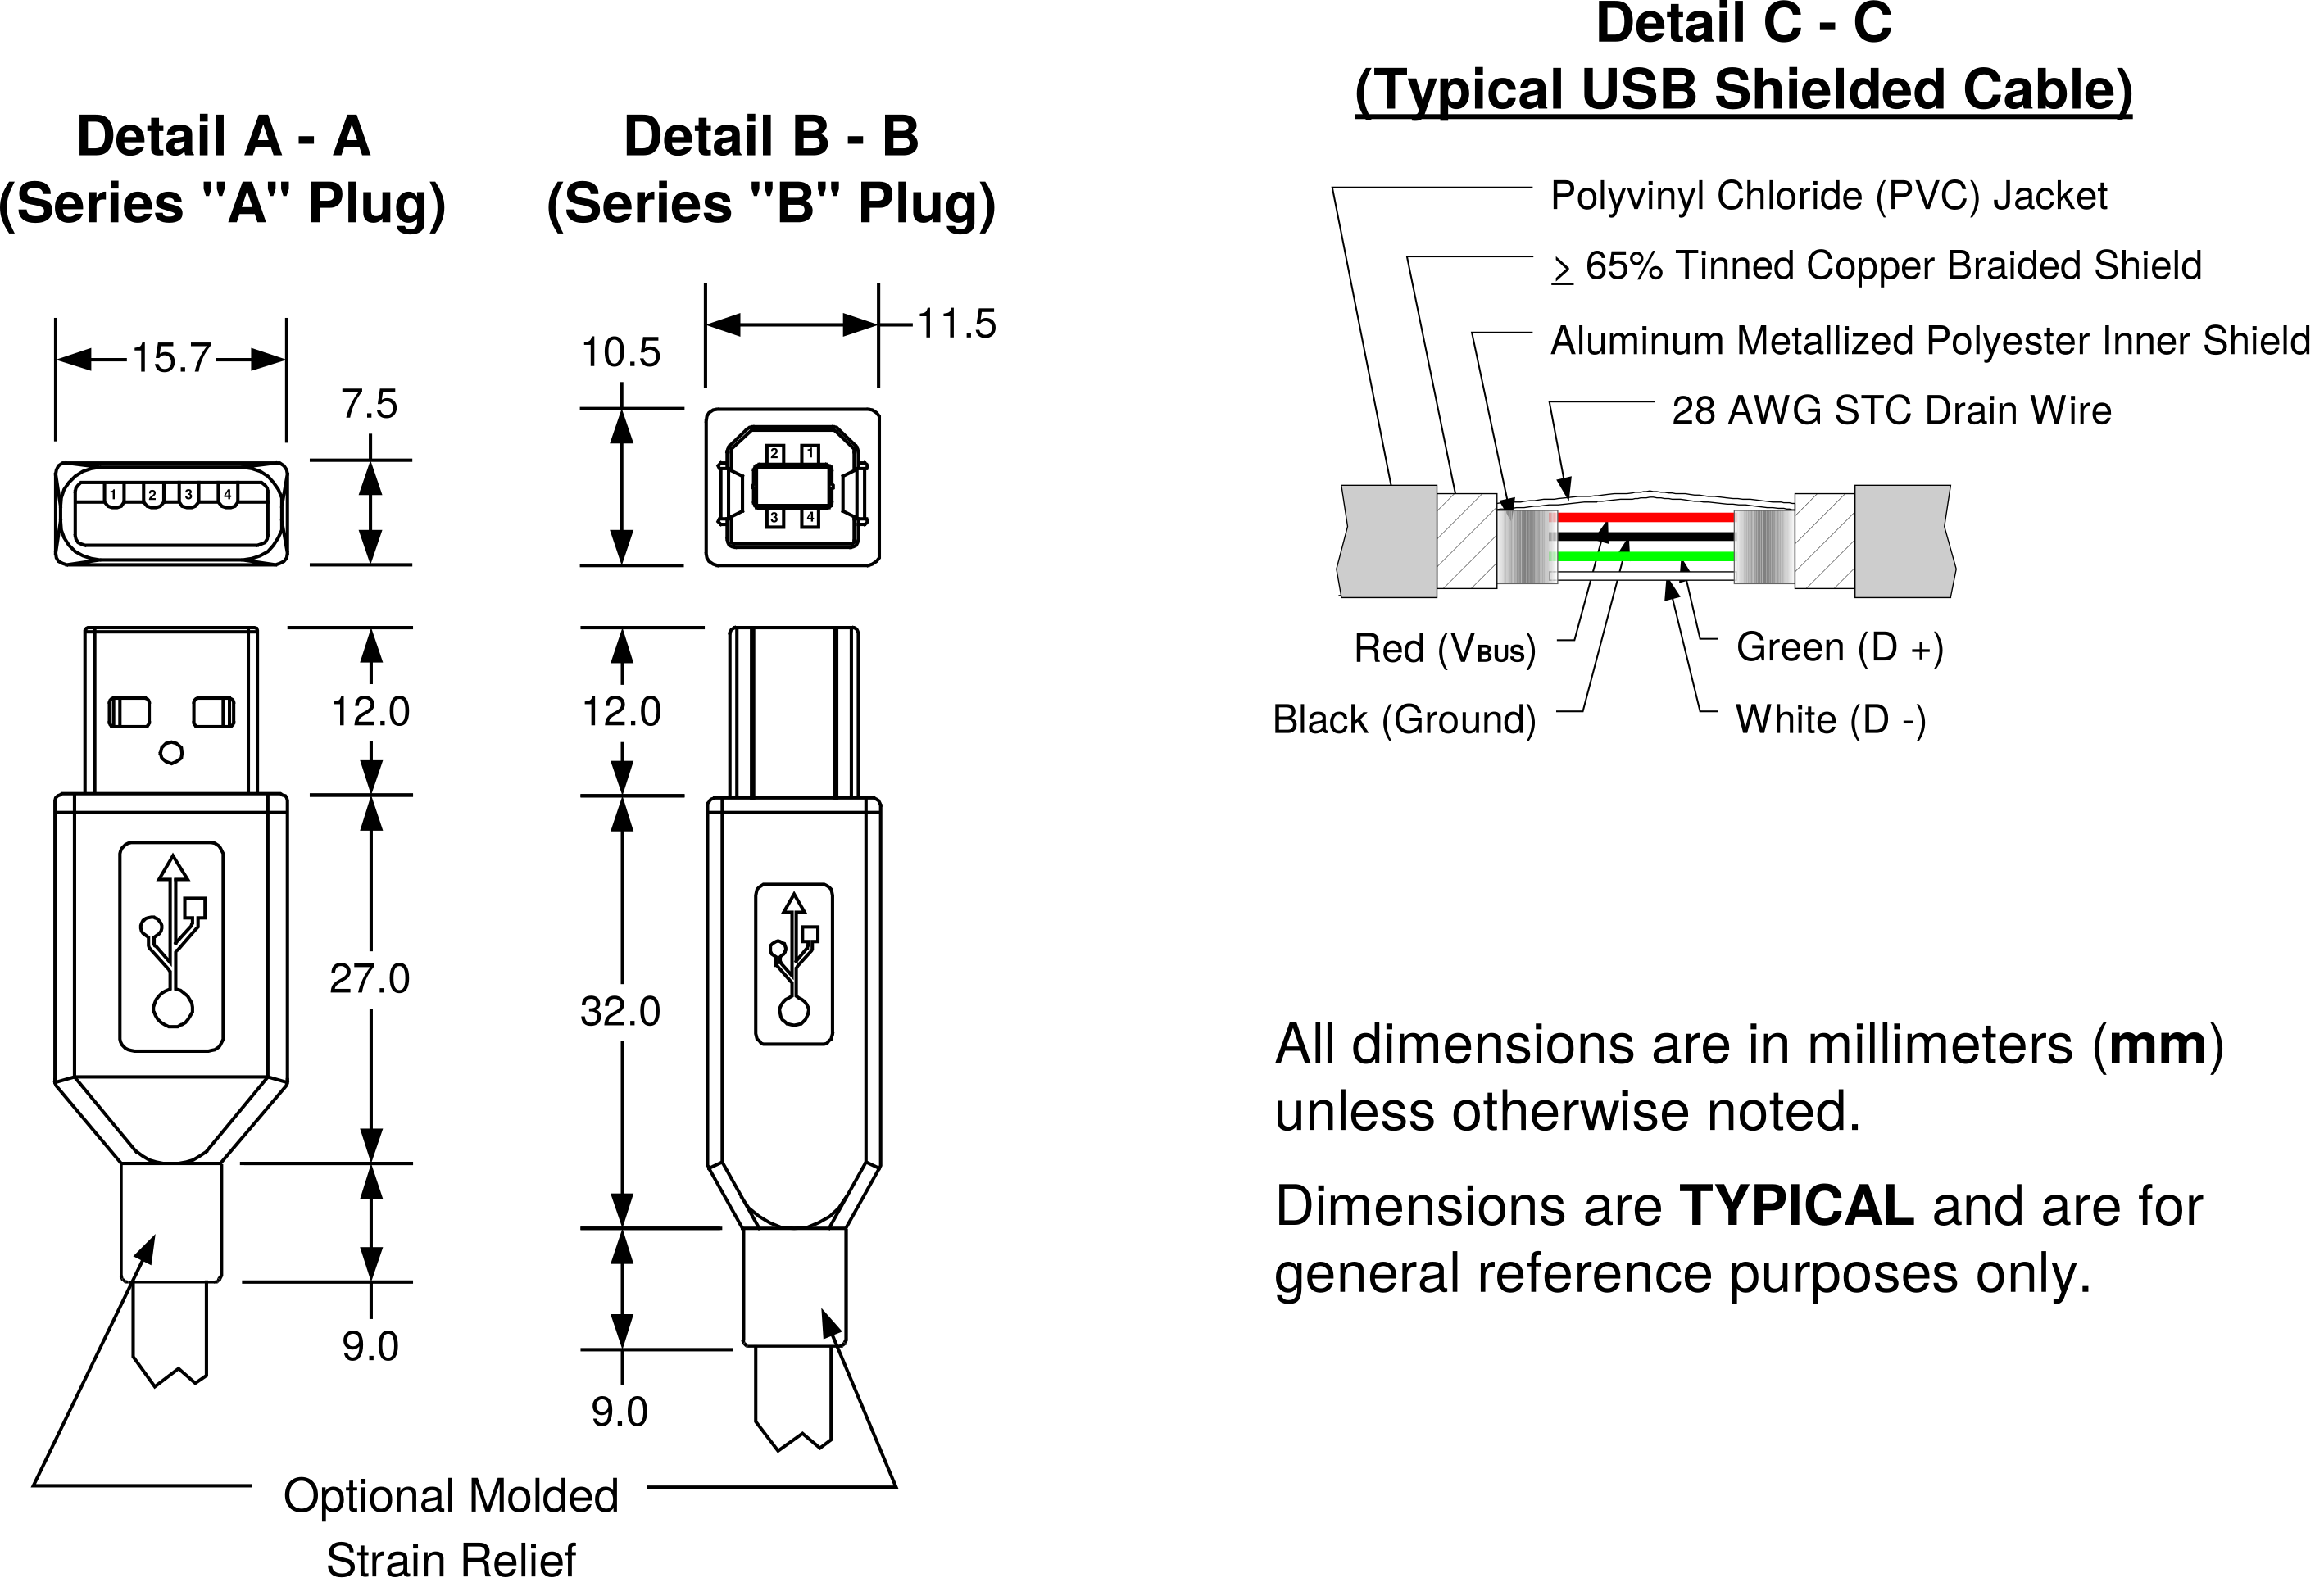
\includegraphics[width=0.9\textwidth]{usbcablea.png}
					\end{figure}}
			\end{frame}
			\begin{frame}{USB - Tipo de transferencias}
					Existen 4 tipos de transferencia los cuales difieren en cómo es transmitida la información, la dirección que posee, el tamaño máximo, acceso al bus, tiempos de latencia, manejo de errores y la secuencia de requerimiento de datos
				\begin{itemize}
					\item Transferencias de Control
					\item Transferencias de Interrupción
					\item Transferencias de Bultos
					\item Transferencias Isocrónicas
				\end{itemize}
				%AQUI me quedé
			\end{frame}
			\begin{frame}{USB - Especificaciones eléctricas}
				\begin{itemize}
					\item Existen 3 velocidades de señalización posibles: 480 Mbit/s denominada high-speed, 12 Mbit/s para full-speed y 1.5 Mbit/s con low-speed.
					\item Se utiliza señal diferencial con un esquema de codificación NRZI (inversión de no retorno a zero).
					\item Los conductores de energía, $V_{BUS}$ y GROUND poseen \si{5} y \SI{0}{\volt} respectivamente.
					\item Los conductores de datos son diferenciales y están polarizados de forma tal que pueda ser identificada la velocidad de operación y la conexión/desconexión de dispositivos.
				\end{itemize}
			\end{frame}
			\begin{frame}{USB - Codificación NRZI}
				\begin{figure}
					\begin{tikzpicture}[scale=.6]
						\begin{scope}[transform shape,node distance=0.1,text width=20]
							\setcounter{wavecount}{0}
							\newwave{Data}
								\bit{0}{1}
								\bit{1}{2}
								\bit{0}{1}
								\bit{1}{1}
								\bit{0}{1}
								\bit{1}{1}
								\bit{0}{3}
								\bit{1}{1}
								\bit{0}{2}
								\bit{1}{2}
								\bit{0}{1}
							\newwave{NRZI - J}
								\bit{0}{3}
								\bit{1}{2}
								\bit{0}{2}
								\bit{1}{1}
								\bit{0}{1}
								\bit{1}{2}
								\bit{0}{1}
								\bit{1}{3}
								\bit{0}{1}
							\newwave{NRZI - K}
								\bit{1}{3}
								\bit{0}{2}
								\bit{1}{2}
								\bit{0}{1}
								\bit{1}{1}
								\bit{0}{2}
								\bit{1}{1}
								\bit{0}{3}
								\bit{1}{1}
						\end{scope}
						\begin{scope}[on background layer]
							\foreach \x in {1,2,...,16}{
								\draw[dashed,black!20] (\x.3,0) -- (\x.3,\value{wavecount}+1);}
						\end{scope}
					\end{tikzpicture}
				\end{figure}
			\end{frame}
	\section{Implementación}
		\subsection{Arquitectura del sistema}
			\begin{frame}{Arquitectura del sistema realizado}
				\only<1>{
					\begin{center}
						\begin{tikzpicture}[scale=1.3\textwidth/\paperwidth,>=latex]
							\begin{scope}
								\begin{scope}[transform shape,node distance=2]
									\node[bloque]	(fpga)	[]{FPGA};
									\node[bloque]	(pc) 	[left=of fpga]	{PC};
									\draw[->,thick] (pc.15) -- node (usbd+) [above]	{D+} (pc.15 -| fpga.west);
									\draw[->,thick] (fpga.195) -- node (usbd-) [below]	{D-} (fpga.195 -| pc.east);
									\node[node distance=.4] (usb text) [above=of usbd+] {USB};
								\end{scope}
								\begin{scope}
									\node[rectangle,rounded corners,draw=black,dashed,fit=(usb text)(usbd+)(usbd-)(fpga.south west)(pc.east)](usb){};
								\end{scope}
							\end{scope}
						\end{tikzpicture}
					\end{center}}
				\only<2->{
					\begin{center}
						\begin{tikzpicture}[scale=1,>=latex]
							\begin{scope}
								\begin{scope}[transform shape,node distance=2]
									\only<2>{\node[bloque]	(cy)				{Interfaz};}
									\only<3->{\node[bloque]	(cy)				{Interfaz\\\alert{Cypress FX2LP}};}
									\only<-3>{\node[bloque]	(fpga)	[right=of cy]{FPGA};}
									\only<4->{\node[bloque]	(fpga)	[right=of cy]{FPGA\\\alert{Xilinx Spartan VI}};}
									\only<-4>{\node[bloque]	(pc) 	[left=of cy]	{PC};}
									\only<5->{\node[bloque]	(pc) 	[left=of cy]	{PC\\\alert{libusb}};}
									\draw[->,thick] (pc.15) -- node (usbd+) [above]	{D+} (pc.15 -| cy.west);
									\draw[->,thick] (cy.195) -- node (usbd-) [below]	{D-} (cy.195 -| pc.east);
									\draw[<->,thick] (cy.15) -- node (data) [above] {Datos} (cy.15 -| fpga.west);
									\draw[->,thick]  (fpga.195) -- node (ctrl) [below] {Control} (fpga.195 -| cy.east);
									\node[node distance=.4] (usb text) [above=of usbd+] {USB};
								\end{scope}
								\begin{scope}
									\node[rectangle,rounded corners,draw=black,dashed,fit=(usb text)(usbd+)(usbd-)(cy.south west)(pc.east)](usb){};
								\end{scope}
							\end{scope}
						\end{tikzpicture}
					\end{center}}
			\end{frame}
		\subsection{Configuración del puente}
			\begin{frame}{Placa de desarrollo utilizada para la interfaz}
				\centering
				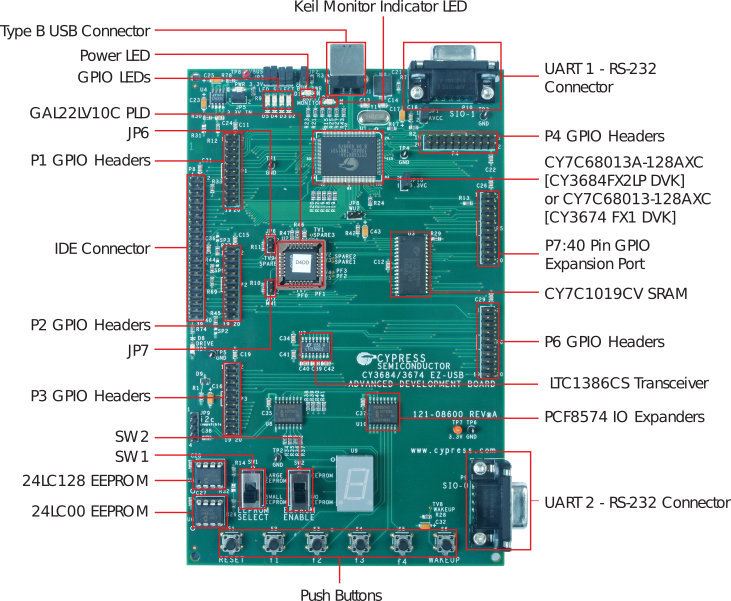
\includegraphics[height=0.8\textheight]{cy3684}
			\end{frame}
			\begin{frame}{El circuito integrado FX2LP}
				\centering
				\begin{tikzpicture}[scale=.58,>=latex]
					\begin{scope}[align=center,transform shape]
						\node	(aux1) {};
						\node[core,minimum height=95] (mis)	[left=of aux1,anchor=north east] {MIS};
						\node[core]	(ram) [right=of aux1,anchor=north west,text width=30] {16 kB RAM};
						\node[perif,text width=60] (xcvr) [left=of mis]	{Transceptor USB};
						\node[core,minimum size=60,text width=50] (uc) [above=of aux1] {8051 Mejorado};			
						\node[perif,node distance=2.9] (pll) [left=of uc] {PLL};
						\node	(aux2)	[right=of ram.south]{};				
						\node[core]	(bus)	[right=of aux2,rotate=90,anchor=north west]	{Bus de datos y direcciones};
						\node[perif]	(i2c)	[right=of bus.south east,anchor=north west]	{I2C};
						\node[perif]	(gpif)	[right=of bus.south west,anchor=south west] {GPIF};
						\node[perif,text width=40] (fifo) [below=of gpif] {4 kB FIFO};
						\node 			(aux3)	[right=of fifo]	{};
						\node 			(aux5) 	[left=of ram] {};
						\draw[<->]	(mis) -- (xcvr);
						\draw[<->]	(ram) -- (ram -| mis.east);
						\draw[<->]	(fifo) -- (fifo -| mis.east);
						\draw[<->]	(ram) to (ram -| bus.north);
						\draw[<->]	(uc) to (uc -| bus.north);
						\draw[<-]	(xcvr) to (xcvr |- pll.south);
						\draw[->]	(pll) to (uc);
						\draw[<->]	(i2c) to (i2c -| bus.south);
						\draw[<->]	(gpif) to (gpif -| bus.south);
						\draw[]		(fifo) -| (aux5.center);
					\end{scope}
					\begin{scope}[on background layer]
						\node[contenedor] (fx2) [fit=(pll)(xcvr)(uc)(bus)(mis)(ram)(fifo)(gpif)(i2c)(aux3)]{};
					\end{scope}
					\begin{scope}[transform shape]
						\node[text width=40,align=center]	(xtal)	[left=of pll]{Xtal \SI{24}{\mega\hertz}};
						\node	(host)	[left=3of xcvr]	{PC};
						\draw[<->,ultra thick] (host) -- node [above,text width=70,midway,align=center]{Comunicación USB} (xcvr);
						\draw[->] (xtal) to (pll);
						\draw[<->,ultra thick] (bus.240) -- node [above,align=center,text width=80] {Datos, direcciones y entradas adicionales}(bus.240 -| fx2.east);
						\draw[<->,thick] (gpif) to (gpif -| fx2.east);
						\draw[<->,thick] (fifo) to (fifo -| fx2.east);
						\draw[<->,thick] (i2c) to (i2c -| fx2.east);
					\end{scope}
				\end{tikzpicture}
			\end{frame}
			\begin{frame}{Configuración del dispositivo USB}
				\begin{columns}
					\begin{column}{.2\textwidth}
							\begin{tikzpicture}[scale=.32,align=center,>=latex]				\begin{scope}[node distance=0.4,transform shape]
									\node[buf]	(ep2b1)	[anchor=north]		{\ep{1}{2}{512}};
									\node[buf]	(ep2b2)	[below=of ep2b1]	{\ep{2}{2}{512}};
									\node[obuf]	(ep4b1) [below=of ep2b2]	{\ep{1}{4}{512}};
									\node[buf]	(ep4b2) [below=of ep4b1]	{\ep{2}{4}{512}};
									\node[obuf]	(ep6b1)	[below=of ep4b2]	{\ep{1}{6}{512}};
									\node[buf]	(ep6b2)	[below=of ep6b1]	{\ep{2}{6}{512}};
									\node[obuf]	(ep8b1)	[below=of ep6b2]	{\ep{1}{8}{512}};
									\node[buf]	(ep8b2)	[below=of ep8b1]	{\ep{2}{8}{512}};
								\end{scope}
							
								\begin{scope}[node distance=0.4, xshift=90,transform shape]
									\node[buf]	(ep2b3)	[anchor=north]		{\epg{1}{2}{1024}};
									\node[obuf] (ep2b4)	[below=of ep2b3]	{\epg{2}{2}{1024}};
									\node[obuf]	(ep2b5)	[below=of ep2b4]	{\epg{3}{2}{1024}};
									\node[obuf]	(ep8b3)	[below=of ep2b5]	{\ep{1}{8}{512}};
									\node[buf]	(ep8b4)	[below=of ep8b3]	{\ep{2}{8}{512}};
								\end{scope}
							
								\begin{scope}[on background layer,inner sep=1,rounded corners]
									\node[env, fit=(ep2b1)(ep2b2)]			(ep21)	{};
									\node[env, fit=(ep4b1)(ep4b2)]			(ep41)	{};
									\node[env, fit=(ep6b1)(ep6b2)]			(ep61)	{};
									\node[env, fit=(ep8b1)(ep8b2)]			(ep81)	{};
									\node[env, fit=(ep2b3)(ep2b4)(ep2b5)]	(ep22)	{};
									\node[env, fit=(ep8b3)(ep8b4)]			(ep82)	{};
								\end{scope}
							
								\begin{scope}[]
									\node[draw=black,inner sep=2,fit=(ep21)(ep82)](marco){};
								\end{scope}
								\begin{scope}[transform shape,node distance=2.5]
									\draw (marco.north) to (marco.south);
									\node[left=of ep2b1.north east,anchor=north east](add1)	{0xF000};
									\node[left=of ep2b1.south east,anchor=south east](add2)	{0xF1FF};
									\node[left=of ep2b2.north east,anchor=north east](add3)	{0xF200};
									\node[left=of ep4b1.north east,anchor=north east](add4)	{0xF400};
									\node[left=of ep6b1.north east,anchor=north east](add5)	{0xF800};
									\node[left=of ep8b1.north east,anchor=north east](add6)	{0xFC00};
									\node[left=of ep8b2.south east,anchor=south east](add7)	{0xFFFF};
									\draw[dashed] (add1.north west) to (add1.north west -| marco.east);
									\draw[dashed] (add3.north west) to (add3.north west -| ep21.east);
									\draw[dashed] (add4.north west) to (add4.north west -| marco.east);
									\draw[dashed] (add5.north west) to (add5.north west -| marco.east);
									\draw[dashed] (add6.north west) to (add6.north west -| marco.east);
									\draw[dashed] (add7.south west) to (add7.south west -| marco.east);
								\end{scope}
							\end{tikzpicture}
					\end{column}
					\begin{column}{.7\textwidth}
						La configuración de las tuberías de comunicación se definieron con la finalidad de obtener el mayor ancho de banda posible a la entrada.
						\begin{itemize}
							\only<1>{\item Entrada:
								\begin{itemize}
									\item Extremo EP2
									\item Transferencias Isocrónicas
									\item 1024 Bytes máximo por transferencia
									\item 3 Buffers
								\end{itemize}}
							\only<2>{\item Salida:
								\begin{itemize}
									\item Extremo EP8
									\item Transferencia por bultos
									\item 512 Butes por transferencia
									\item 2 Buffers
								\end{itemize}}
						\end{itemize}
					\end{column}
				\end{columns}
			\end{frame}
			\begin{frame}{Cypress Software Development Kit}
				\begin{columns}
					\begin{column}{.2\textwidth}
						\begin{tikzpicture}[scale=.42]
							\begin{scope}[transform shape,node distance=1,>=latex]
								\node[mealy]	(start)	[]	{Iniciar: Reset \\ \verb~main();~ };
								\node[moore]	(init)	[below=of start]	{Inicia Variables de Estado}
									edge[<-,thick] (start);
								\node[moore]	(us1)	[below=of init]		{ \verb~TD\_Init();~ }
									edge[<-,thick]	(init);
								\node[moore]	(EI)	[below=of us1]	{Habilita\\Interrupciones}
									edge[<-,thick](us1);
								\node[node distance=0.7]			(aux1)	[below=of EI] 	{};
								\draw[<-,thick](aux1.base) to (EI);
								\node[moore,node distance=.5]	(poll)	[below=of aux1]	{\verb~TD\_Poll();~ }
									edge[<-,thick](aux1.base);
								\node[ask]		(pr1)	[below=of poll]	{Paquete de Setup}
									edge[<-,thick](poll);
								\node[moore]	(setup)	[right=of pr1]	{\verb~SetupComand();~ };
								\draw[->,thick] (setup) |- (aux1.base);
								\node[]			(aux2)	[below=of pr1]	{};
								\draw[->,thick]	(pr1) -- node[above,near start]{Si} (setup);
								\draw[thick]	(pr1) -- node[left,near start]{No}	(aux2.base);
								\node[node distance=2.5](aux3)	[left=of aux2] {};
								\draw[thick]	(aux2.base) -- (aux3.base);
								\draw[->,thick]	(aux3.base)	|-	(aux1.base);
							\end{scope}
						\end{tikzpicture}
					\end{column}
					\begin{column}{.6\textwidth}
						\begin{itemize}
							\item El programa inicia al comienzo del main();
							\item Inicia todas las variables de estado
							\item TD\_Init ejecuta la configuración del usuario
							\item El usuario debe configurar las interrupciones que desea habilitar. Al salir de TD\_Init, el programa habilita todas (\verb~EA=1~)
							\item Finalmente, se ejecuta las instrucciones que el usuario programa de manera específica
							\item Además, se ejecutan las funciones que controlan el USB.
						\end{itemize}
					\end{column}
				\end{columns}
			\end{frame}
		\subsection{Circuito sintetizado}
			\begin{frame}{La placa de desarrollo MOJO v3}
				\begin{columns}
					\begin{column}{.43\textwidth}
						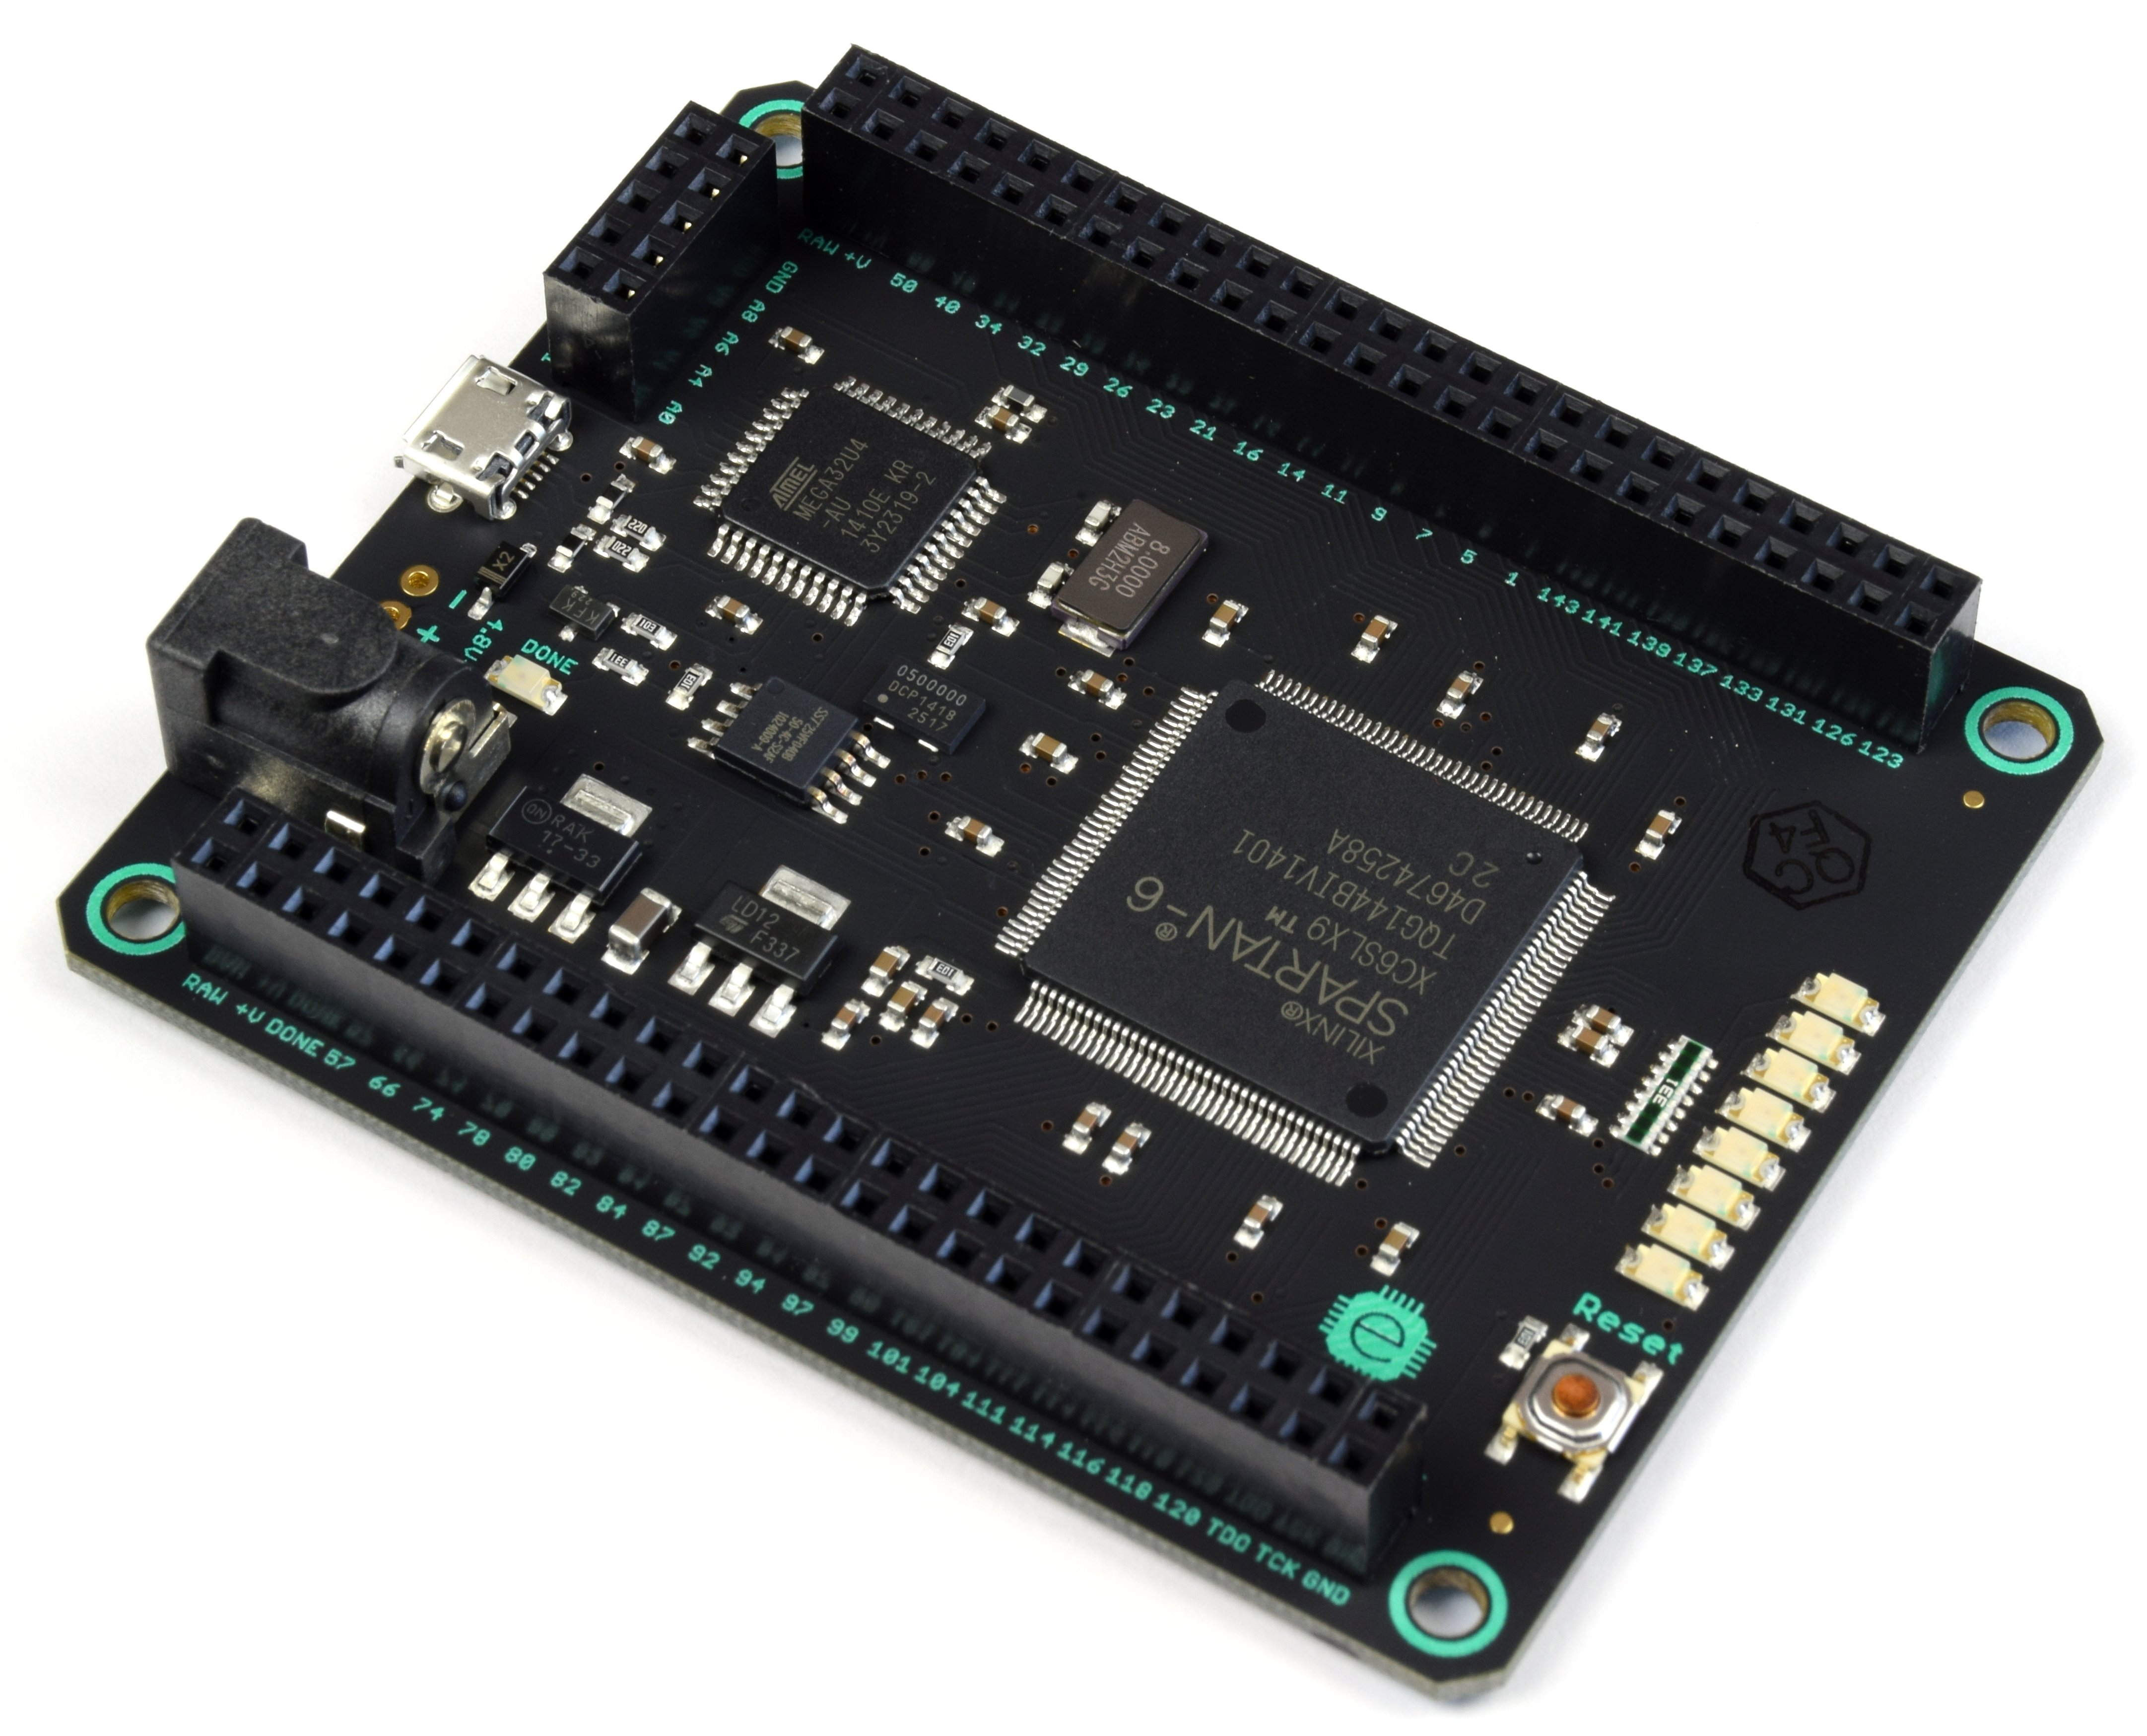
\includegraphics[width=\textwidth]{MojoIso.png}
					\end{column}
					\begin{column}{.55\textwidth}
						\begin{itemize}
							\item FPGA Spartan 6 XC6SLX9 de Xilinx
							\item 84 pines IO digitales
							\item 8 entradas analógicas
							\item 8 LEDs de propósito general
							\item 1 pulsador de propósito general
							\item Regulador de voltaje de entrada de 4.8V - 12V
							\item ATmega32U4 para configurar la FPGA y leer los pines analógicos
							\item Bootloader compatible con Arduino
							\item Memoria flash para almacenar la configuración de la FPGA (programación persistente)
						\end{itemize}
					\end{column}
				\end{columns}
			\end{frame}
			\begin{frame}{Estructura interna FPGA}
				\centering
				\begin{tikzpicture}[scale=.58]
					\begin{scope}[transform shape,node distance=5,>=latex,thick]
						\node[simple]	(cypress)		[]	 			{FIFO Esclava};
						\node[simple]	(master)	[right=of cypress]	{Maestro Externo};
						\node[simple,minimum size=70]	(leer)		[right=of master.north west,anchor=north west] {Leer FIFO};
						\node[simple,minimum size=70]	(escribir)	[right=of master.south west,anchor=south west]	{Escribir FIFO};
						\node[simple,node distance=8]	(fifo)		[right=of master]	{FIFO Interna (XLNX core generator)};
						
						\draw[<->]	([yshift=4*110/6]cypress.east) --node [above]{IFCLK} ([yshift=4*110/6]master.west);
						\draw[<->]	([yshift=3*110/6]cypress.east) --node [above]{FD[15:0]} ([yshift=3*110/6]master.west);
						\draw[<-]	([yshift=2*110/6]cypress.east) --node [above]{FIFOADR[1:0]} ([yshift=2*110/6]master.west);
						\draw[->]	([yshift=1*110/6]cypress.east) --node [above]{EP2\_EMPTY} ([yshift=1*110/6]master.west);
						\draw[->]	([yshift=0*110/6]cypress.east) --node [above]{EP8\_FULL} ([yshift=0*110/6]master.west);
						\draw[<-]	([yshift=-1*110/6]cypress.east) --node [above]{SLOE} ([yshift=-1*110/6]master.west);
						\draw[<-]	([yshift=-2*110/6]cypress.east) --node [above]{SLWR} ([yshift=-2*110/6]master.west);
						\draw[<-]	([yshift=-3*110/6]cypress.east) --node [above]{SLRD} ([yshift=-3*110/6]master.west);
						\draw[<-]	([yshift=-4*110/6]cypress.east) --node [above]{PKTEND} ([yshift=-4*110/6]master.west);
						
						\draw[<-] (leer) -- node[above]{SLWR} (master.east |- leer);
						\draw[<-] ([yshift=-1*80/7]leer.east) -- node[above]{EMPTY}([yshift=-1*80/7]fifo.west |- leer);
						\draw[->] ([yshift=1*80/7]leer.east) -- node[above]{RD\_EN}([yshift=1*80/7]fifo.west |- leer);
						
						\draw[<-] (escribir) -- node[above]{SLRD} (master.east |- escribir);
						\draw[<-] ([yshift=-1*80/7]escribir.east) -- node[above]{FULL}([yshift=-1*80/7]fifo.west |- escribir);
						\draw[->] ([yshift=1*80/7]escribir.east) -- node[above]{WR\_EN}([yshift=1*80/7]fifo.west |- escribir);			
						
						\draw[<-]	([yshift=1*110/6]fifo.west) --node [above]{DIN[15:0]} ([yshift=1*110/6]master.east);
						\draw[->]	([yshift=0*110/6]fifo.west) --node [above]{DOUT[15:0]} ([yshift=0*110/6]master.east);
						\draw[<-]	([yshift=-1*110/6]fifo.west) --node [above]{VALID} ([yshift=-1*110/6]master.east);
						
						\node[node distance=.4] (fpga) [above=of leer] {FPGA};
					\end{scope}
					\begin{scope}[on background layer]
						\node[rectangle,rounded corners,dashed,fit=(master)(leer)(fpga)(fifo)(escribir),draw=black]{};
					\end{scope}
				\end{tikzpicture}
			\end{frame}
			\begin{frame}{Interfaz - FPGA}
				\centering
				\begin{tikzpicture}[scale=.95]
					\begin{scope}[transform shape,node distance=5,>=latex]
						\node[simple]	(fifo)		[]	 			{FIFO Esclava};
						\node[simple]	(master)	[right=of fifo]	{Maestro Externo};
						\draw[<->,thick]	([yshift=5*110/6]fifo.east) --node [above]{IFCLK} ([yshift=5*110/6]master.west);
						\draw[<->,thick]	([yshift=4*110/6]fifo.east) --node [above]{FD[15:0]} ([yshift=4*110/6]master.west);
						\draw[<-,thick]	([yshift=3*110/6]fifo.east) --node [above]{FIFOADR[1:0]} ([yshift=3*110/6]master.west);
						\draw[->,thick]	([yshift=2*110/6]fifo.east) --node [above]{FLAGA} ([yshift=2*110/6]master.west);
						\draw[->,thick]	([yshift=1*110/6]fifo.east) --node [above]{FLAGB} ([yshift=1*110/6]master.west);
						\draw[->,thick]	([yshift=0*110/6]fifo.east) --node [above]{FLAGC} ([yshift=0*110/6]master.west);
						\draw[->,thick]	([yshift=-1*110/6]fifo.east) --node [above]{FLAGD} ([yshift=-1*110/6]master.west);
						\draw[<-,thick]	([yshift=-2*110/6]fifo.east) --node [above]{SLOE} ([yshift=-2*110/6]master.west);
						\draw[<-,thick]	([yshift=-3*110/6]fifo.east) --node [above]{SLWR} ([yshift=-3*110/6]master.west);
						\draw[<-,thick]	([yshift=-4*110/6]fifo.east) --node [above]{SLRD} ([yshift=-4*110/6]master.west);
						\draw[<-,thick]	([yshift=-5*110/6]fifo.east) --node [above]{PKTEND} ([yshift=-5*110/6]master.west);
					\end{scope}
				\end{tikzpicture}
			\end{frame}
			\begin{frame}{Máquina de estados algorítmica de la interfaz}
				\centering
				\begin{tikzpicture}[scale=.35]
					\begin{scope}[transform shape,node distance=1,>=latex]
						\node[moore]	(idle)	[]	{--idle:\\SLRD='1';\\SLOE='1';\\SLWR='1';\\FIFOADR="ZZ";};
						\node[ask]	(pr1)	[below=of idle]	{EP2\_empty='0'}
						edge[<-] (idle);
						\node[ask]	(pr2)	[right=of pr1]	{write\_req='1'};
						\node[ask]	(pr3)	[below=of pr2]	{EP8\_full='0'};
						\node[moore]	(radr)	[left=of pr1]		{--read address:\\SLRD='1';\\SLOE='1';\\SLWR='1';\\FIFOADR="00";};
						
						\draw[->](pr1) -- node [above,near start]{No}(radr);
						\draw[->](pr1) -- node [above,near start]{Si} (pr2);
						
						\node[node distance=0.8](aux1)[right=of pr2]{};
						\draw[->](pr2) -- node[left,near start]{Si}(pr3);
						\draw[->](pr2.east) |- node[above,near end]{No}(aux1.base);
						
						\node[moore]	(rnempty)	[left=of radr]	{--read no empty:\\SLRD='0';\\SLOE='0';\\SLWR='1';\\FIFOADR="00";}
						edge[<-](radr);
						\node[moore](rread)[below=of rnempty]{--read read:\\SLRD='1';\\SLOE='0';\\SLWR='1;\\FIFOADR="00";}
						edge[<-](rnempty);
						
						\node[moore](wadr)	[left=of pr3]	{--write address:\\SLRD='1';\\SLOE='1';\\SLWR='1';\\FIFOADR="11";};
						\node[node distance=.8](aux2)[right=of pr3]{};
						\draw[->](pr3) -- node[above,near start]{Si} (wadr);
						\draw[->](pr3) -- node[above,near start]{No}(aux2.base) -| (aux1.base);
						
						\node[moore](wnfull)[below=of wadr] {--write no full:\\SLRD='1';\\SLOE='1';\\SLWR='0';\\FIFOADR="11";}
						edge[<-] (wadr);
						\node[node distance=.5](aux3)[left=of wnfull]{};
						\draw[->] (wnfull) -- (aux3.base);
						\node[moore,node distance=.5](wwrite)[left=of aux3] {--write write:\\SLRD='1';\\SLOE='1';\\SLWR='1';\\FIFOADR="11";}
						edge[<-] (aux3.base);
						
						\node[ask](pr4)[below=of wwrite] {fifo\_valid='1'}
						edge[<-] (wwrite);
						\node[moore](wend)[left=of pr4] {--write end:\\SLRD='1';\\SLOE='1';\\SLWR='1';\\FIFOADR="11";};
						\node[node distance=.7] (aux4) [right=of pr4]{}; 
						\draw[->]	(pr4) -- node[above,near start]{Si} (wend);
						\draw[->](pr4) -- node[above] {No} (aux4.base);
						\draw[->](aux4.base) -- (aux3.base);
						
						\node[ask](pr5)[below=of wend] {write\_req='1'}
						edge[<-] (wend);
						\node[ask](pr6)[right=of pr5] {EP2\_empty='0'};
						\node[node distance=.8] (aux5) [left=of rread] {};
						\node[node distance=.8] (aux7) [left=of pr5] {};
						\draw[->] (rread) -- (aux5.base);
						\draw[->] (pr5)	-- node[above,near start] {No} (aux7.base);
						\draw[->] (pr5) -- node[above,near start] {Si} (pr6);
						
						\node[node distance=.8] (aux6)[below=of pr6] {};
						\draw[->] (pr6) -| node[above,near start] {Si} (wnfull);
						\draw[->] (pr6) -- node[left]{No} (aux6.base) -| (aux7.base);
						\draw[->] (aux7.base) |- (aux5.base);
						
						\node[node distance=.8] (aux8) [above=of idle] {};
						\draw[->] (aux8.base) -- (idle);
						\draw[->] (aux5.base) |- (aux8.base);
						\draw[->](aux1.base) |- (aux8.base);
						
					\end{scope}
				\end{tikzpicture}
			\end{frame}
			\begin{frame}{Maquinas de estado hacia la memoria FIFO interna}
				\begin{columns}
					\begin{column}{.5\textwidth}
						\centering
						\begin{tikzpicture}[scale=.53]
							\begin{scope}[transform shape,node distance=1,>=latex]
								\node[moore] (idle) {--idle:\\RE\_EN='0';};
								\node[node distance=.6](aux0)[above=of idle]{};
								\node[ask]	(pr1)	[below=of idle]{\tiny{SLWR='0'-$>$'1'}}
									edge[<-] (idle);
								\node[ask] (pr2) [below=of pr1]{\scriptsize{FIFO\_empty='1'}};
								\node[node distance=.8](aux1)[left=of pr1]{};
								\draw[->] (pr1) -- node[left] {Si} (pr2);
								\draw[->] (pr1) -- node[above,near start]{No} (aux1.base);
								\draw[->] (aux1.base) |- (aux0.base) -- (idle);
								
								\node[moore](rden)[below=of pr2]{--read enable:\\RD\_EN='1'};
								\node[node distance=.8] (aux2) [left=of pr2] {};
								\draw[->] (pr2) -- node[above,near start]{Si} (aux2.base);
								\draw[->] (pr2) -- node[left,near start] {No} (rden);
								\draw[->] (aux2.base) -- (aux1.base);
								
								\node[node distance=.8] (aux3) [below=of rden]{};
								\draw[->] (rden) -- (aux3.base) -| (aux2.base); 
							\end{scope}
						\end{tikzpicture}
					\end{column}
					\begin{column}{.5\textwidth}
						\centering
						\begin{tikzpicture}[scale=.5]
							\begin{scope}[transform shape,node distance=1,>=latex]
								\node[moore] (idle) {--idle:\\WR\_EN='0';};
								\node[node distance=.6](aux0)[above=of idle]{};
								\node[ask]	(pr1)	[below=of idle]{\tiny{SLRD='0'-$>$'1'}}
									edge[<-] (idle);
								\node[ask] (pr2) [below=of pr1]{\scriptsize{FIFO\_FULL='1'}};
								\node[node distance=.8](aux1)[left=of pr1]{};
								\draw[->] (pr1) -- node[left] {Si} (pr2);
								\draw[->] (pr1) -- node[above,near start]{No} (aux1.base);
								\draw[->] (aux1.base) |- (aux0.base) -- (idle);
								
								\node[moore](rden)[below=of pr2]{--write enable:\\WR\_EN='1'};
								\node[node distance=.8] (aux2) [left=of pr2] {};
								\draw[->] (pr2) -- node[above,near start]{Si} (aux2.base);
								\draw[->] (pr2) -- node[left,near start] {No} (rden);
								\draw[->] (aux2.base) -- (aux1.base);
								
								\node[node distance=.8] (aux3) [below=of rden]{};
								\draw[->] (rden) -- (aux3.base) -| (aux2.base); 
							\end{scope}
						\end{tikzpicture}
					\end{column}
				\end{columns}
			\end{frame}
		\subsection{Circuito de interconexión}
			\begin{frame}{Circuito de interconexión}
				\begin{itemize}
					\only<1-2>{\item Versión 1\\
						\only<1>{\centering
							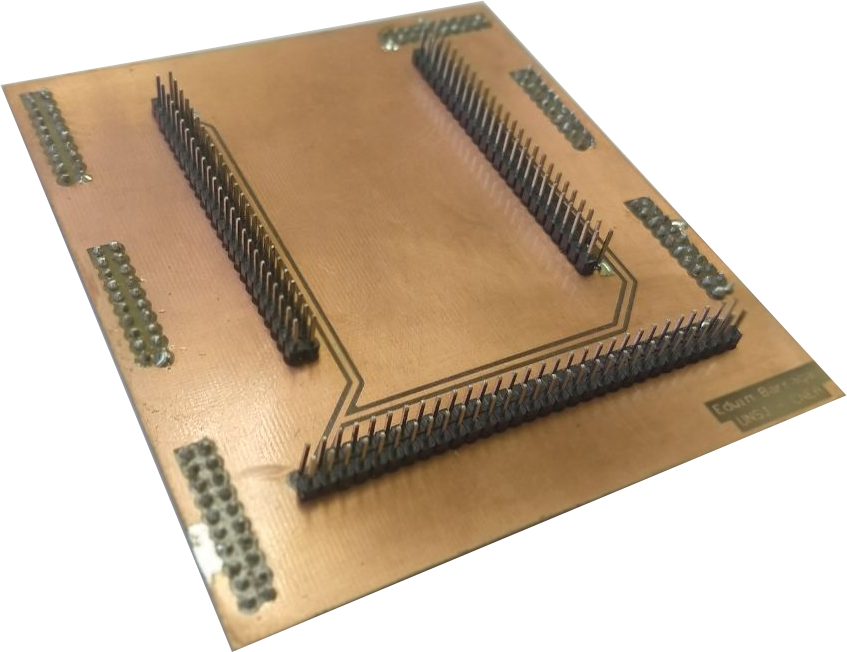
\includegraphics[width=.6\textwidth]{61v1anverso}}
						\only<2>{\centering
							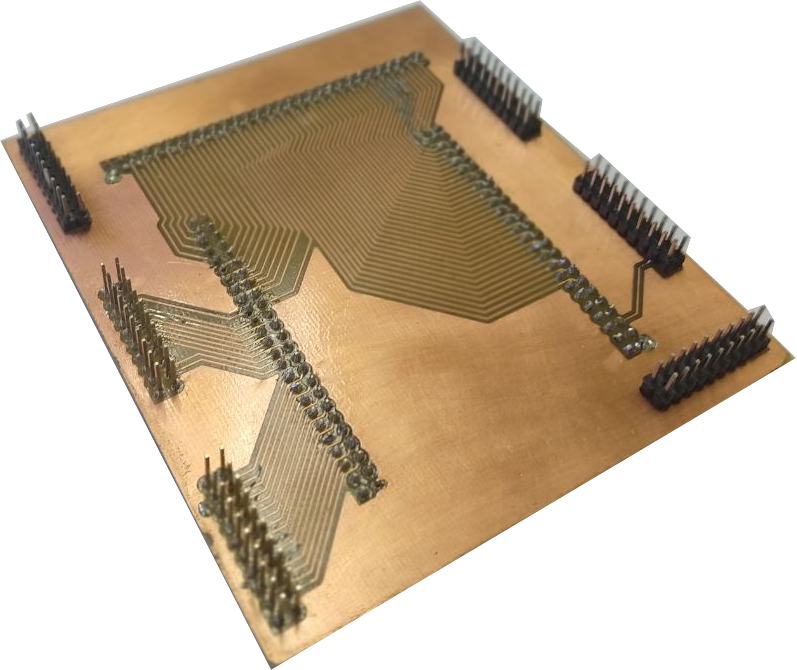
\includegraphics[width=.6\textwidth]{62v1reverso}}}
						
					\only<3-4>{\item Versión 2\\
						\only<3>{\centering
							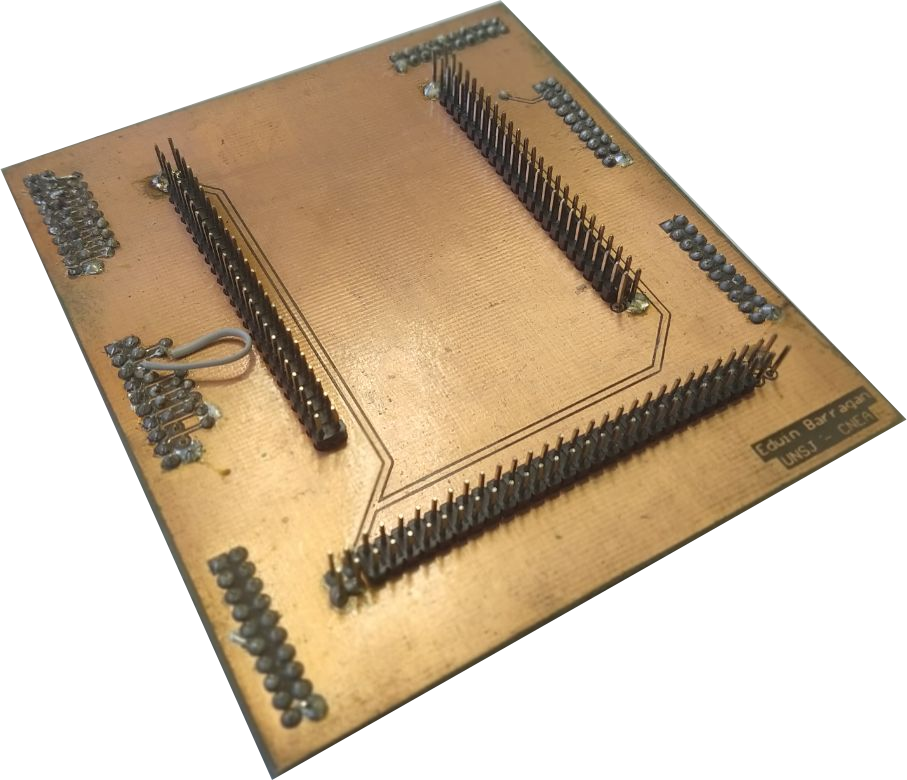
\includegraphics[width=.6\textwidth]{63v2anverso}}
						\only<4>{\centering
							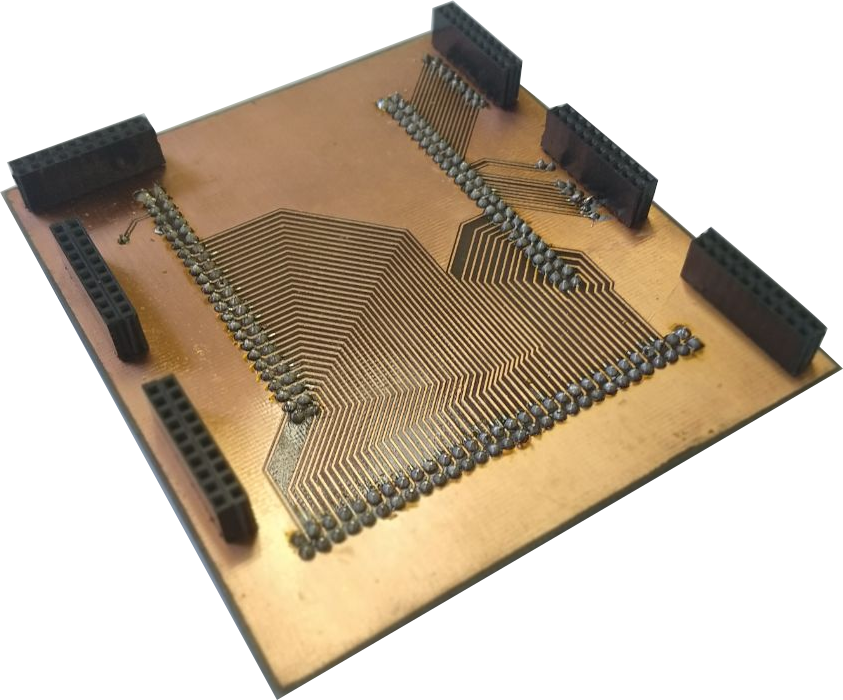
\includegraphics[width=.6\textwidth]{64v2reverso}}}

					\only<5-6>{\item Versión 3\\
						\only<5>{\centering
							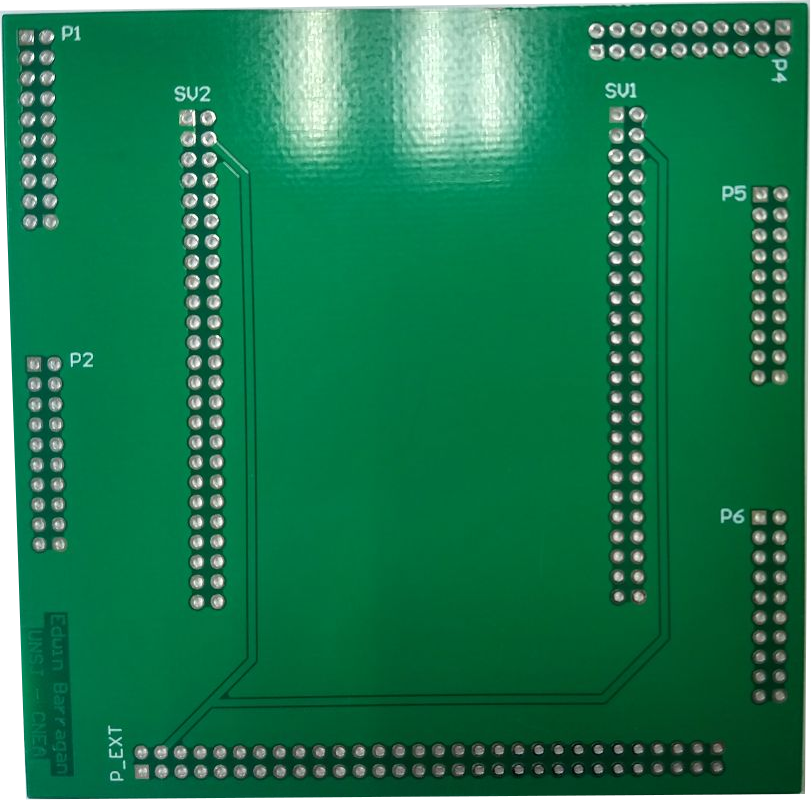
\includegraphics[width=.6\textwidth]{65v3anverso}}
						\only<6>{\centering
							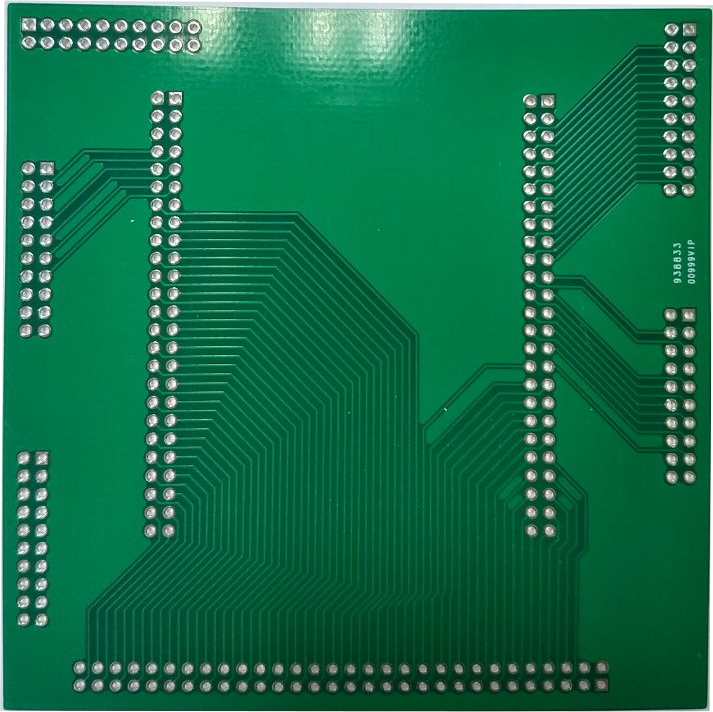
\includegraphics[width=.6\textwidth]{66v3reverso}}}
				\end{itemize}
			\end{frame}
			\begin{frame}{Sistema completo}
				\centering
				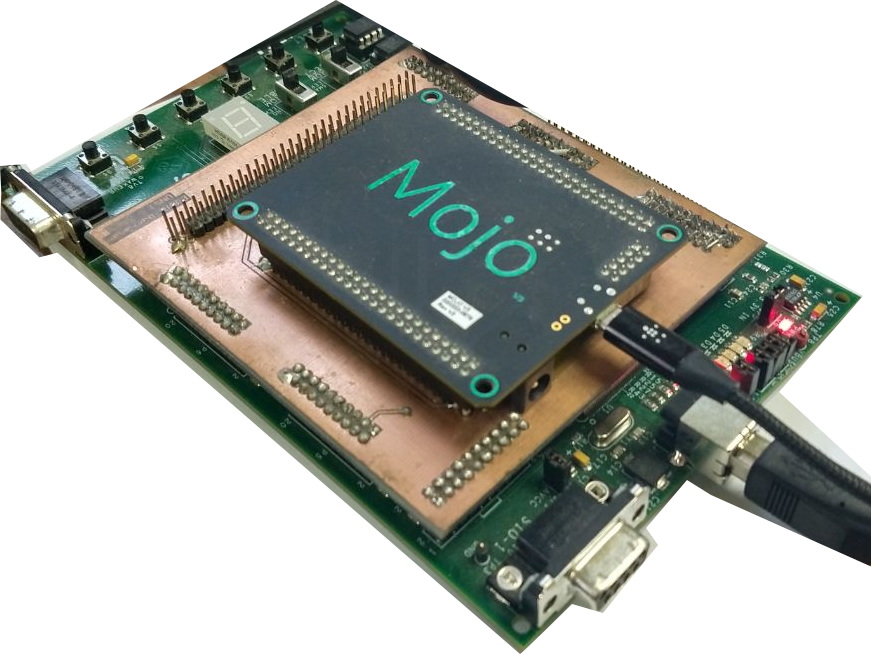
\includegraphics[width=.6\textwidth]{fisico}
			\end{frame}
	\section{Evaluación y validación}
		\subsection{Test benchs de VHDL}
			\begin{frame}{Test bench}
				\only<1>{El sistema fue simulado con el objetivo de corroborar el correcto funcionamiento del sistema, cómo así también detectar fallas en la descripción realizada y obtener una forma de depuración de lo realizado.}
				\only<2>{
					\centering
					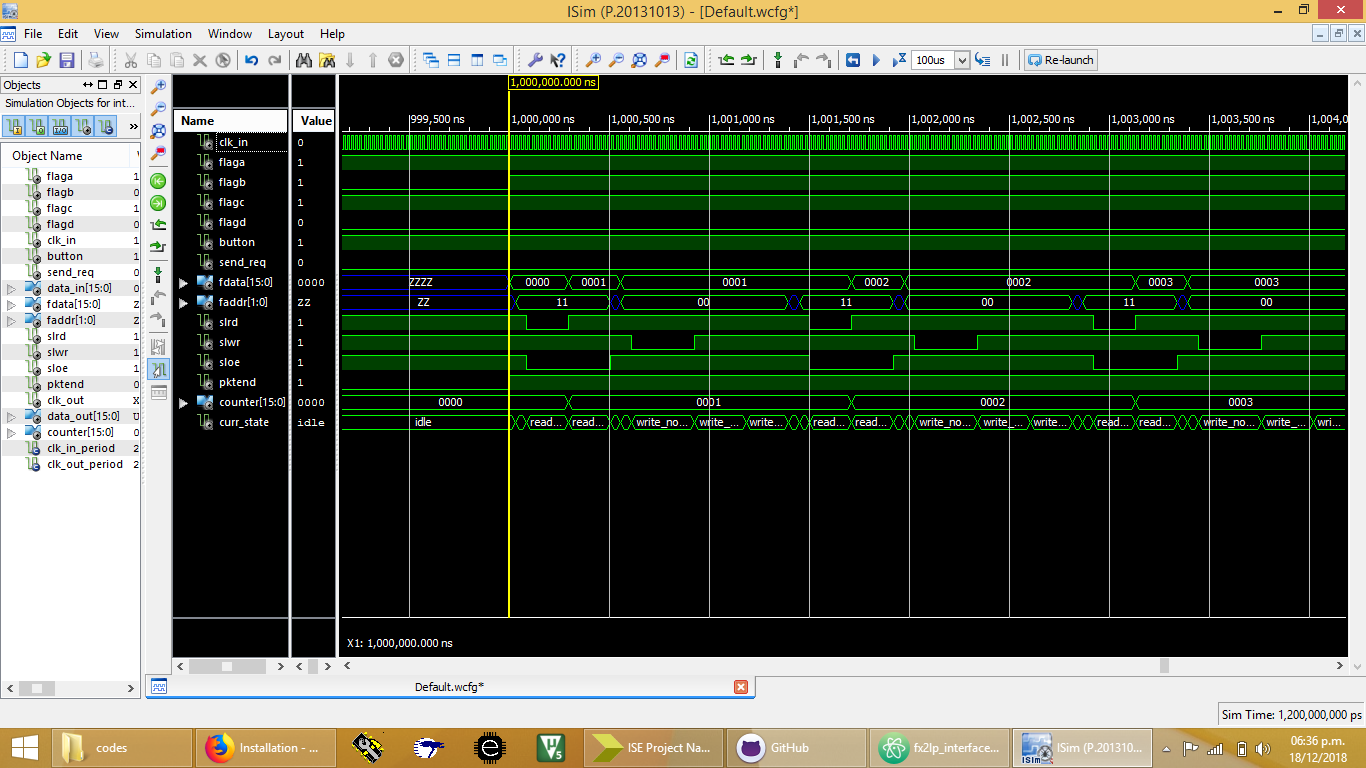
\includegraphics[width=\textwidth]{51tbinicio}}
				\only<3>{
					\centering
					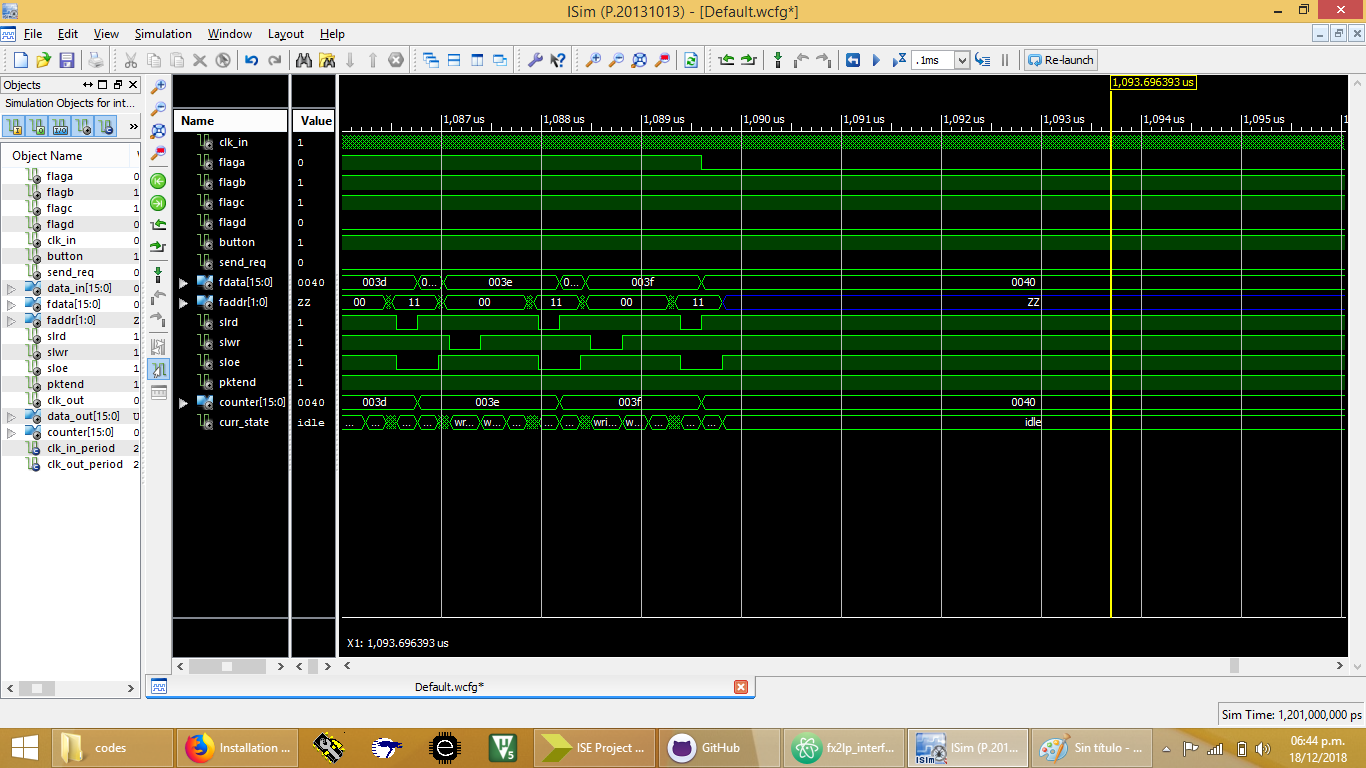
\includegraphics[width=\textwidth]{52tbfinalflaga}}
				\only<4>{
					\centering
					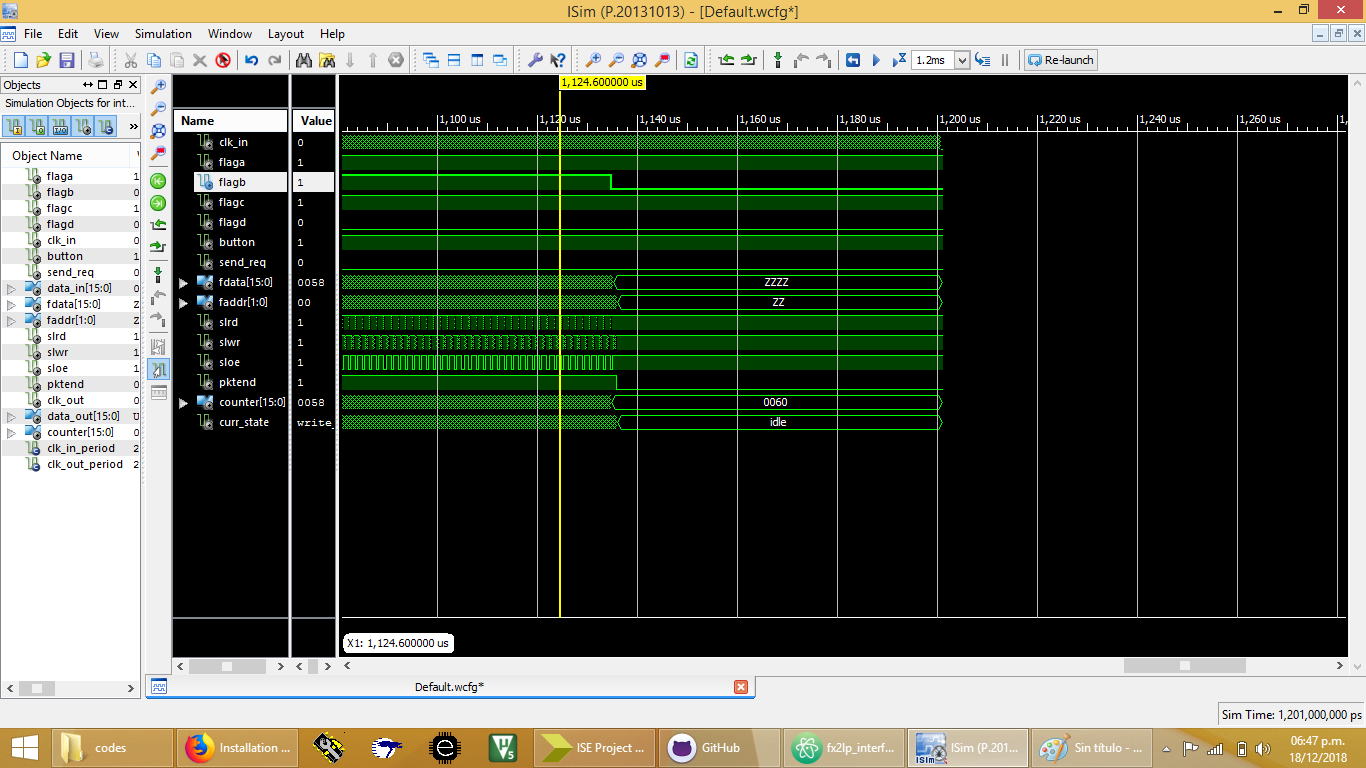
\includegraphics[width=\textwidth]{53tbfinalflagb}}
				\only<5>{
					\centering
					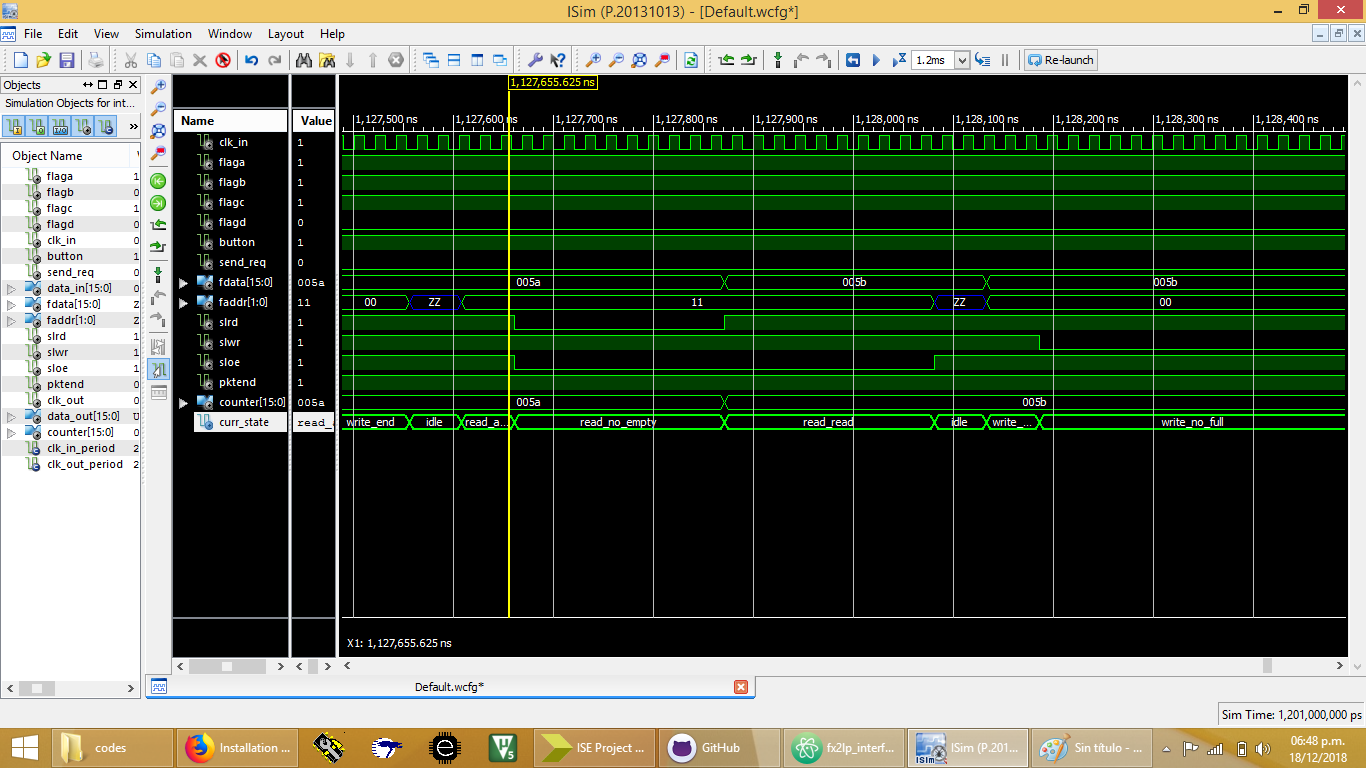
\includegraphics[width=\textwidth]{54tbmea}}
			\end{frame}
		\subsection{Depuración de firmware del puente}
			\begin{frame}{Debug Cypress}
				
			\end{frame}
		\subsection{Biblioteca de PC}
			\begin{frame}{\texttt{libusb-1.0}}
				
			\end{frame}
		\subsection{Programas de prueba}
			\begin{frame}{Esquemas de prueba}
				
			\end{frame}
		\subsection{Elementos de VHDL utilizados para depuración}
			\begin{frame}{Flip-Flop para eco}
				
			\end{frame}
			\begin{frame}{ROM con patrón de repetición infinita}
				
			\end{frame}
	\section{Resultados y conclusiones}
		\subsection{Robustez}
			\begin{frame}{Resultados de la prueba de robustez\\de la comunicación}
				
			\end{frame}
		\subsection{Tasa máxima de Transferencia}
			\begin{frame}{Resultados de la prueba de máxima transferencia de datos}
				TODO
			\end{frame}
		\subsection{Trabajo futuro}
			\begin{frame}{Lo que falta...}
				
			\end{frame}
			\begin{frame}{Consultas}
				
			\end{frame}
			\begin{frame}[c]
				\centering
				\alert {Muchas gracias}
			\end{frame}
			
			\begin{frame}{Material Adicional}
				\centering
				Respaldo y cosas que no entren
			\end{frame}
			\scriptsize{
			\lstinputlisting[language=C]{./codes/bridge.c}}
\end{document}